\chapter{Search for invisibly decaying VBF produced Higgs bosons in Run 1 prompt data}
\label{chap:prompt}
%Introduction to selection and challenges of jets+met, e.g. trigger, \ac{QCD}
As described in \ChapterRef{chap:theory}, searches for invisible Higgs boson decays are well motivated by their sensitivity to new physics, such as \ac{DM}. Because the invisible branching of an \ac{SM} 125 \GeV\, Higgs boson is very small, any observation made of invisible Higgs boson decays at the \LHC would be evidence for physics beyond the \ac{SM}. This chapter describes the search for invisible Higgs boson decays using data taken by CMS in 2012 with a promptly reconstructed trigger developed specifically for this analysis. The total integrated luminosity collected with this trigger that was certified for use in physics analyses was 19.5\invfb~. The analysis was published in \ReferenceRef{Chatrchyan:2014tja}.

\section{Event selection}
\label{sec:promptsel}
%describe backgrounds and motivate selection
In signal events it is expected that there will be two jets with a characteristic \ac{VBF} topology and a large amount of \MET. Several background processes, with significantly higher cross-sections than the signal process, can also produce events with these objects present. It is therefore necessary to design selection criteria, known as ``cuts'', to remove as many of these background events from the analysis as possible.

The most significant of these background processes is the production of a vector boson in association with jets, ``V+jets''. Leptonic decays of \PW bosons and \PZ boson decays to neutrinos both produce \MET and, due to the approximately 1000 times higher cross-section for vector boson production than Higgs boson production, there are many events where the associated jets have a \ac{VBF}-like topology. ``V+jets'' backgrounds with a \PW (\PZ) are referred to as ``\PW(\PZ)+jets''.
A further background process that can produce significant numbers of \ac{VBF}-like jets due to its very large cross-section is \ac{QCD} production of multiple jets (``\ac{QCD} multijets''). Whilst these multijet events have very little \MET from real invisible particles, it is possible for significant ``fake'' \MET to be caused by mismeasurement of the jets. The production of two vector bosons or top quarks can also lead to two jets and real \MET, although they have much lower cross-sections than the other background processes and their contribution is not as significant. %??relative cross-section

%trigger requirements and design
\subsection{Trigger}
\label{sec:prompttrig}
The trigger requirements can be viewed as the first stage of the event selection. Their primary role is to reduce the rate of events that must be recorded by the detector whilst retaining the maximum number of signal events. As described in \SectionRef{sec:triggers} the decision whether to keep an event must be made very rapidly, and as a result the object reconstruction algorithms used are less sophisticated, and the available detector resolution is worse, than those offline. The trigger criteria have therefore been chosen to be as loose as possible whilst maintaining the required rate reduction.

To pass the \ac{L1} trigger selection events are required to have \MET$>40$ \GeV. Events are then required to have \METnoMU$>65$\GeV\, and that at least one pair of jets in the event is \ac{VBF}-like to pass the \ac{HLT} selection. The \ac{VBF}-like requirements on the jets consist of requiring their $\eta$ separation, $\Delta\eta_{jj}$, be greater than 3.5, that they are in opposite forward/backward halves of the detector and that they have high invariant mass, $M_{jj}>800 \GeV$. The use of \METnoMU at trigger level ensures that events which are needed for the control regions used in the background estimation techniques described in \SectionRef{sec:promptbkg} are not rejected. Not requiring that the \ac{VBF}-like pair of jets also be the two highest \pt jets reduces inefficiencies caused by different \pt orderings in jets reconstructed by the trigger and by the offline reconstruction. The efficiency for events to pass the trigger as a function of their values of several offline variables is shown in \FigureRef{fig:prompttrigplots}. The measured trigger efficiency is applied as a weight to all \ac{MC} samples.

%trigger efficiency plots from AN-12-403
\begin{figure}
  \subfloat[]{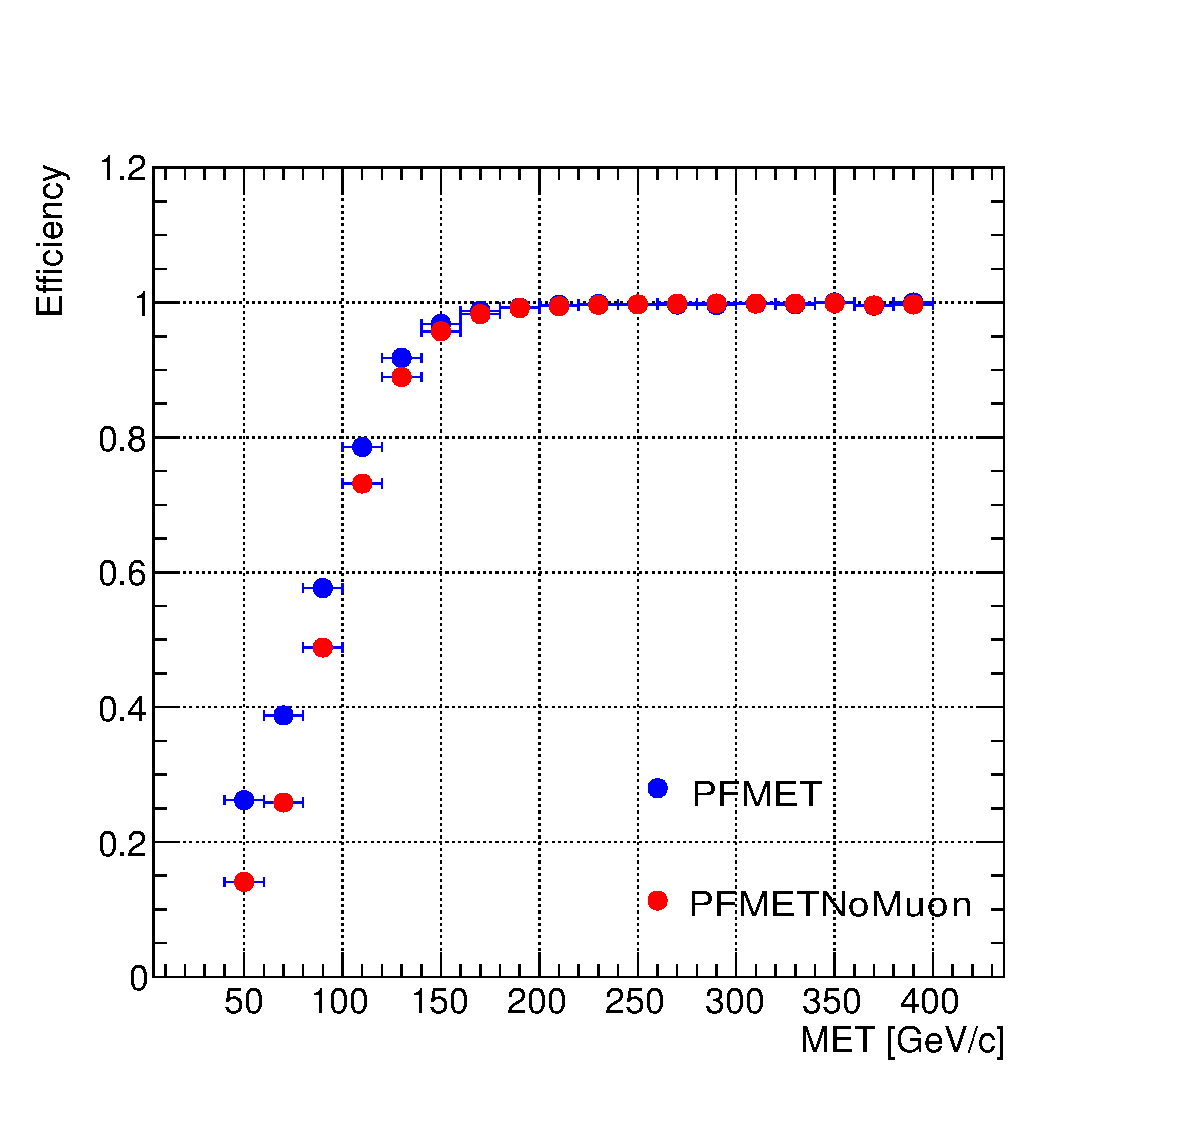
\includegraphics[width=.6\largefigwidth]{plots/prompt/TrigEff_SingleMu_L1ETM40.pdf}}
  \subfloat[]{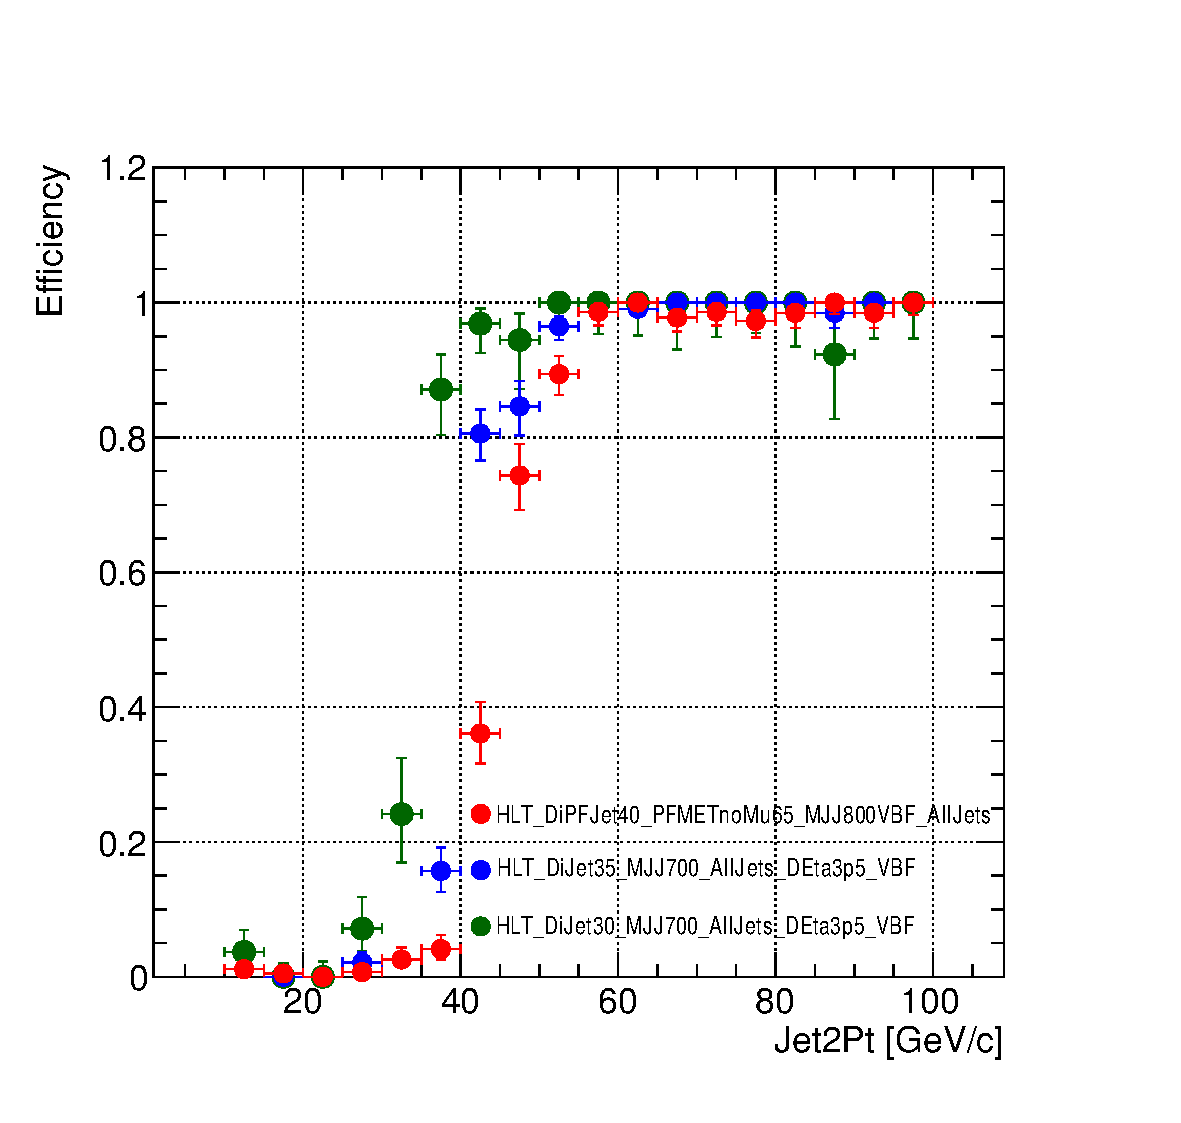
\includegraphics[width=.6\largefigwidth]{plots/prompt/TrigEff_SingleMu_Jet2Pt.pdf}}

  \subfloat[]{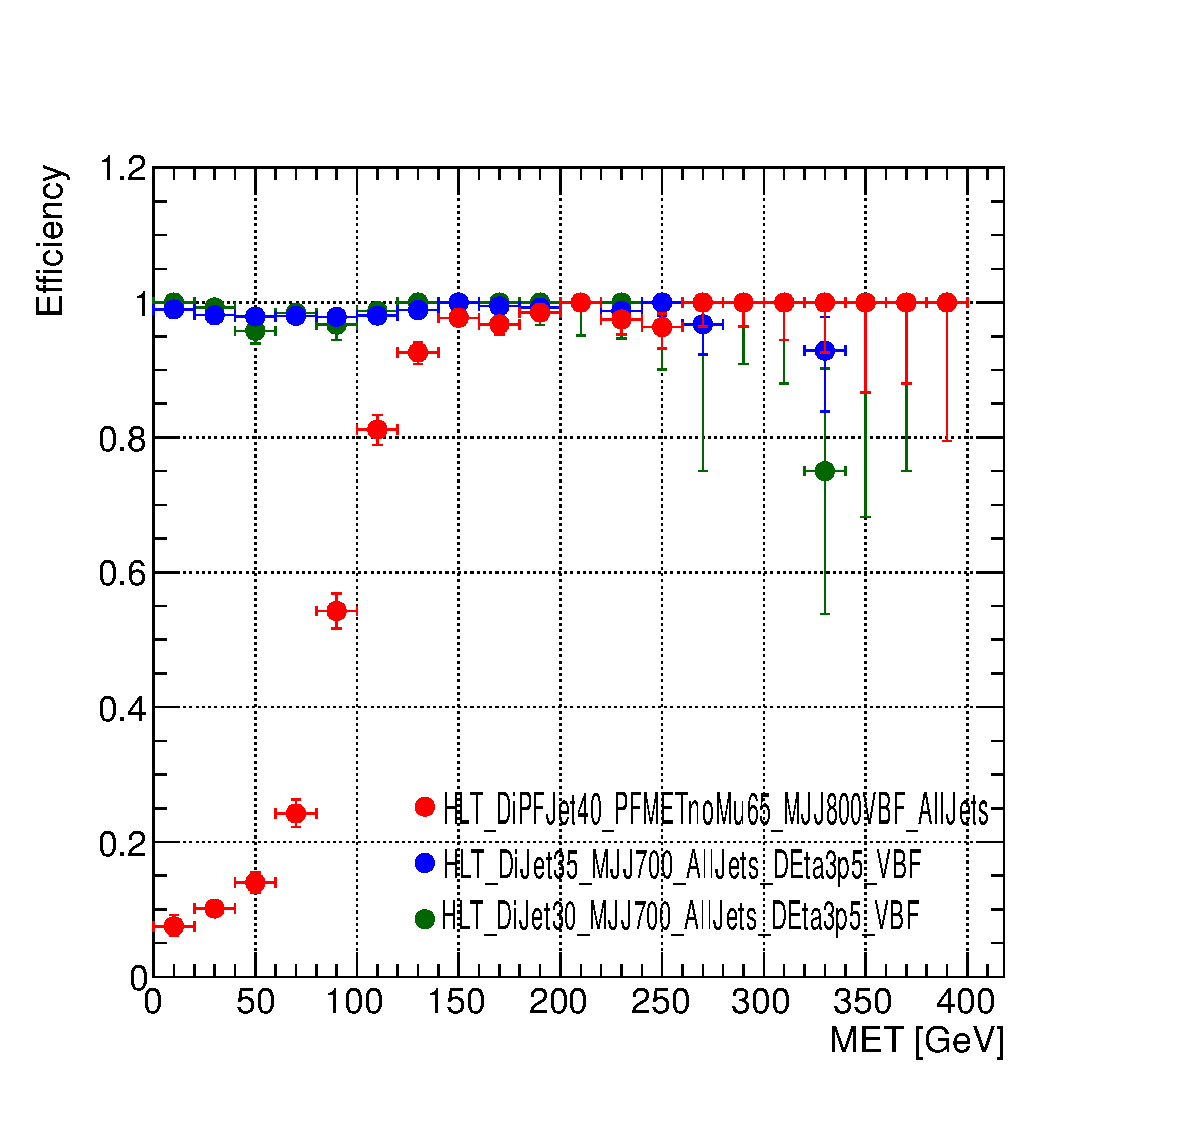
\includegraphics[width=.6\largefigwidth]{plots/prompt/TrigEff_SingleMu_MET.pdf}}
  \subfloat[]{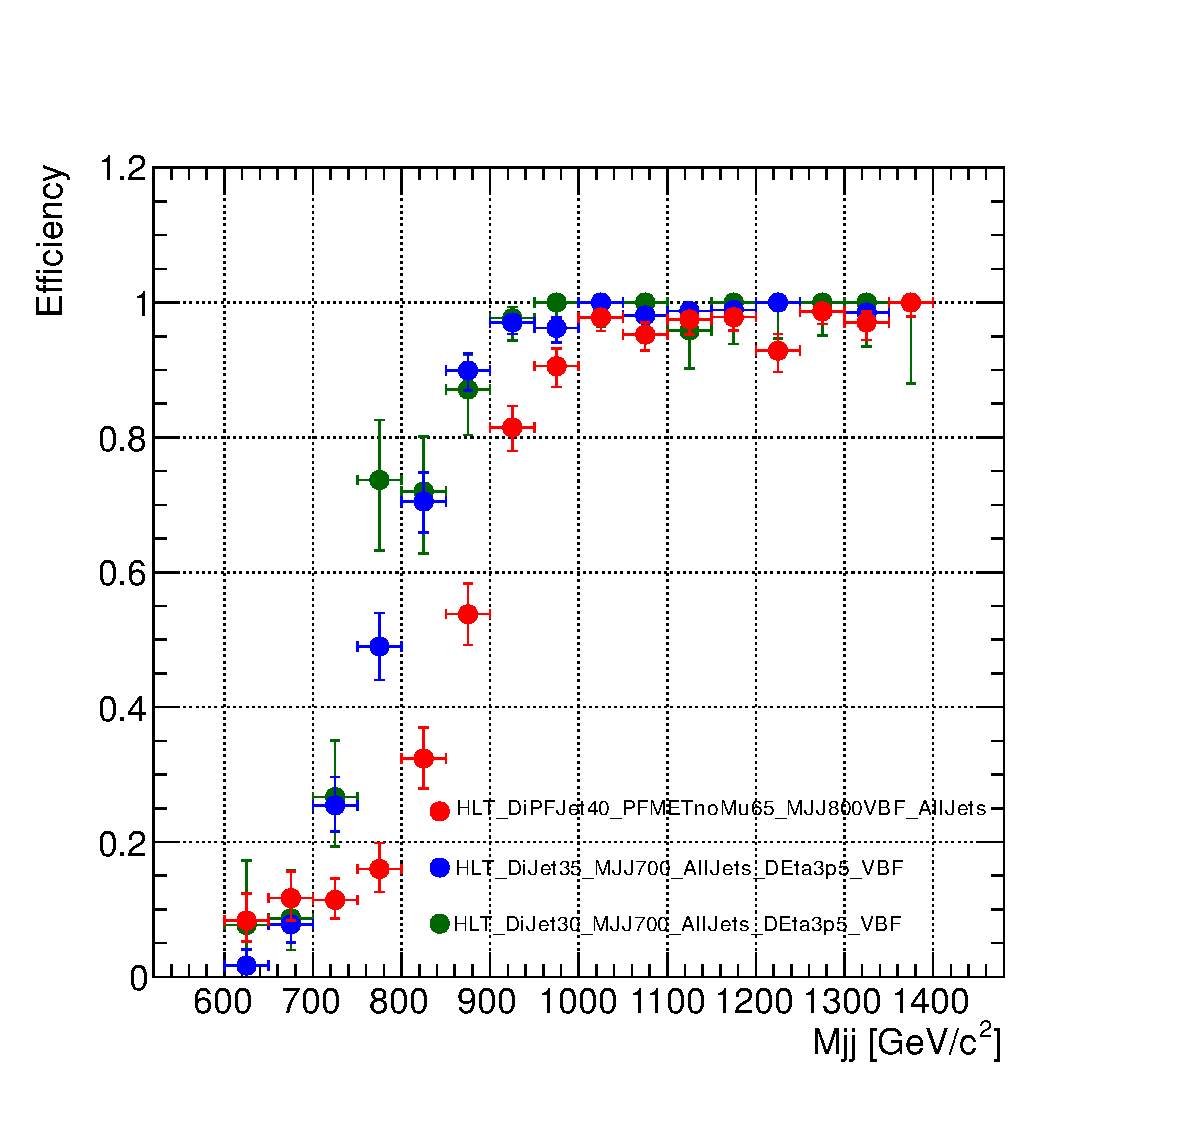
\includegraphics[width=.6\largefigwidth]{plots/prompt/TrigEff_SingleMu_Mjj.pdf}}
  \caption{The trigger efficiency as a function of the values of several offline variables, measured in a sample of events recorded on a single-muon trigger. (a) \ac{L1} trigger efficiency as a function of offline \MET and \METnoMU, (b) \ac{HLT} efficiency as a function of second highest offline jet \pt, (c) \ac{HLT} efficiency as a function of offline \MET, (d) \ac{HLT} efficiency as a function of $M_{jj}$~\cite{ARTICLE:CMSAN-12-403} .}
  \label{fig:prompttrigplots}
\end{figure}

\subsection{Offline selection}
\label{sec:promptofflinesel}
%selection and motivation
The offline selection begins by requiring that events have no veto muons or electrons, as defined in sections \ref{sec:electrons} and \ref{sec:muons}, with \pt$>10$ \GeV. This lepton veto reduces the background from \PW and \PZ boson decays and also from top quarks. The two highest \pt jets in the event are then identified as the VBF tag pair. Tighter versions of the trigger selection are then applied. The tag jets are required to be in opposite forward/backward halves of the detector, to both have \pt$>50$ \GeV\, and $|\eta|<4.7$, to have $M_{jj}>1100$ \GeV and $\Delta\eta_{jj}>4.2$. The \METnoMU is required to be greater than 130 \GeV. Because events with veto muons have been vetoed \METnoMU is in the case of the signal region identical to \MET. However, it is important for background estimation methods that \METnoMU and not \MET is used.

As well as the trigger based selection further cuts are made to reduce the \ac{QCD} multijet background to a level much lower than the V+jets backgrounds. The two tag jets are required to have an azimuthal separation, $\Delta\phi_{jj}<1.0$, since multijet events with \MET due to mismeasurement are most likely to have their jets back-to-back in the detector, i.e. with $\Delta\phi_{jj}=\pi$. Events where there are any jets with \pt$>30$ \GeV\, between the two tag jets in $\eta$ are also vetoed. This \ac{CJV} is motivated by the lack of colour connection, described in \SectionRef{sec:higprod}, between the quarks in VBF production that makes the presence of such jets unlikely in genuine signal events.

The specific values of the cuts on each variable are chosen for three reasons. Firstly, the reconstruction algorithms for some objects are only well validated for certain values of \pt and $\eta$. This consideration decides the threshold for the \ac{CJV} and lepton vetos. Secondly, as can be seen from \FigureRef{fig:prompttrigplots}, the values of the offline variables where the trigger becomes fully efficient are in some cases much higher than the online cut. Because the variables used in the trigger are highly correlated, the offline cuts on all variables used in the trigger were chosen such that the trigger efficiency for the variable at that point is greater than 95\%. The region of phase space remaining after all cuts have been applied is called the signal region.

Finally, the values of the cuts are optimised to provide the best expected limit on \BRinv for a 125 \GeV\, Higgs boson, which is calculated using the method described in \SectionRef{sec:stats} with the background estimation carried out as in \SectionRef{sec:promptbkg} and the systematic uncertainties as described in \SectionRef{sec:promptsyst}. For the tag jet \pt and \MET, no improvement in the expected limit is seen by tightening the cut, so the requirement is at the 95\% efficiency point of the trigger. The full selection gives a $(6.8\pm 0.3)\times 10^{-3}$ efficiency for selecting events from invisible decays of a VBF produced 125 \GeV\, Higgs boson. The distributions and cut values for several of the other variables used are shown in \FigureRef{fig:promptcontrolplots}. 

%discriminating variable plots from HIG-13-030
\begin{figure}
  \subfloat[]{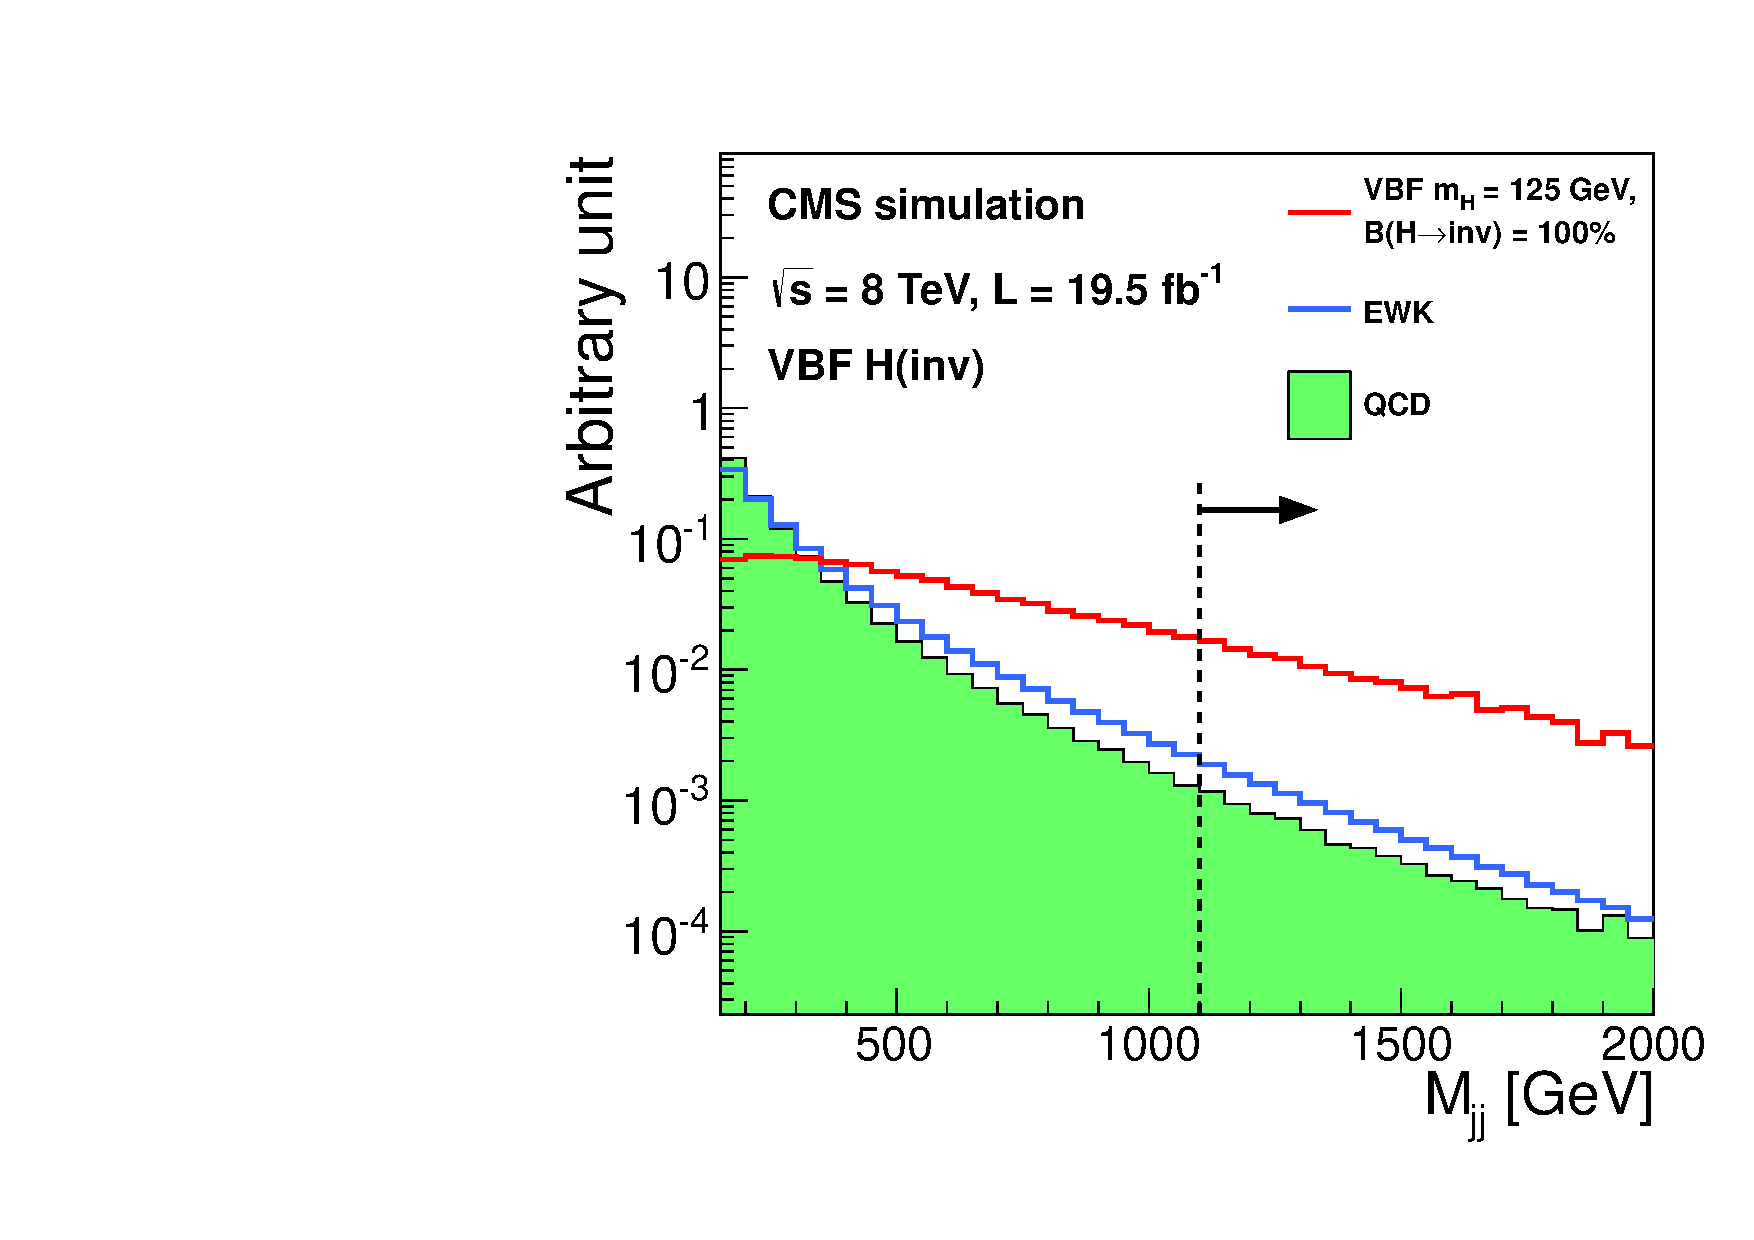
\includegraphics[width=.6\largefigwidth]{plots/prompt/VBF-Dijet-M.pdf}}
  \subfloat[]{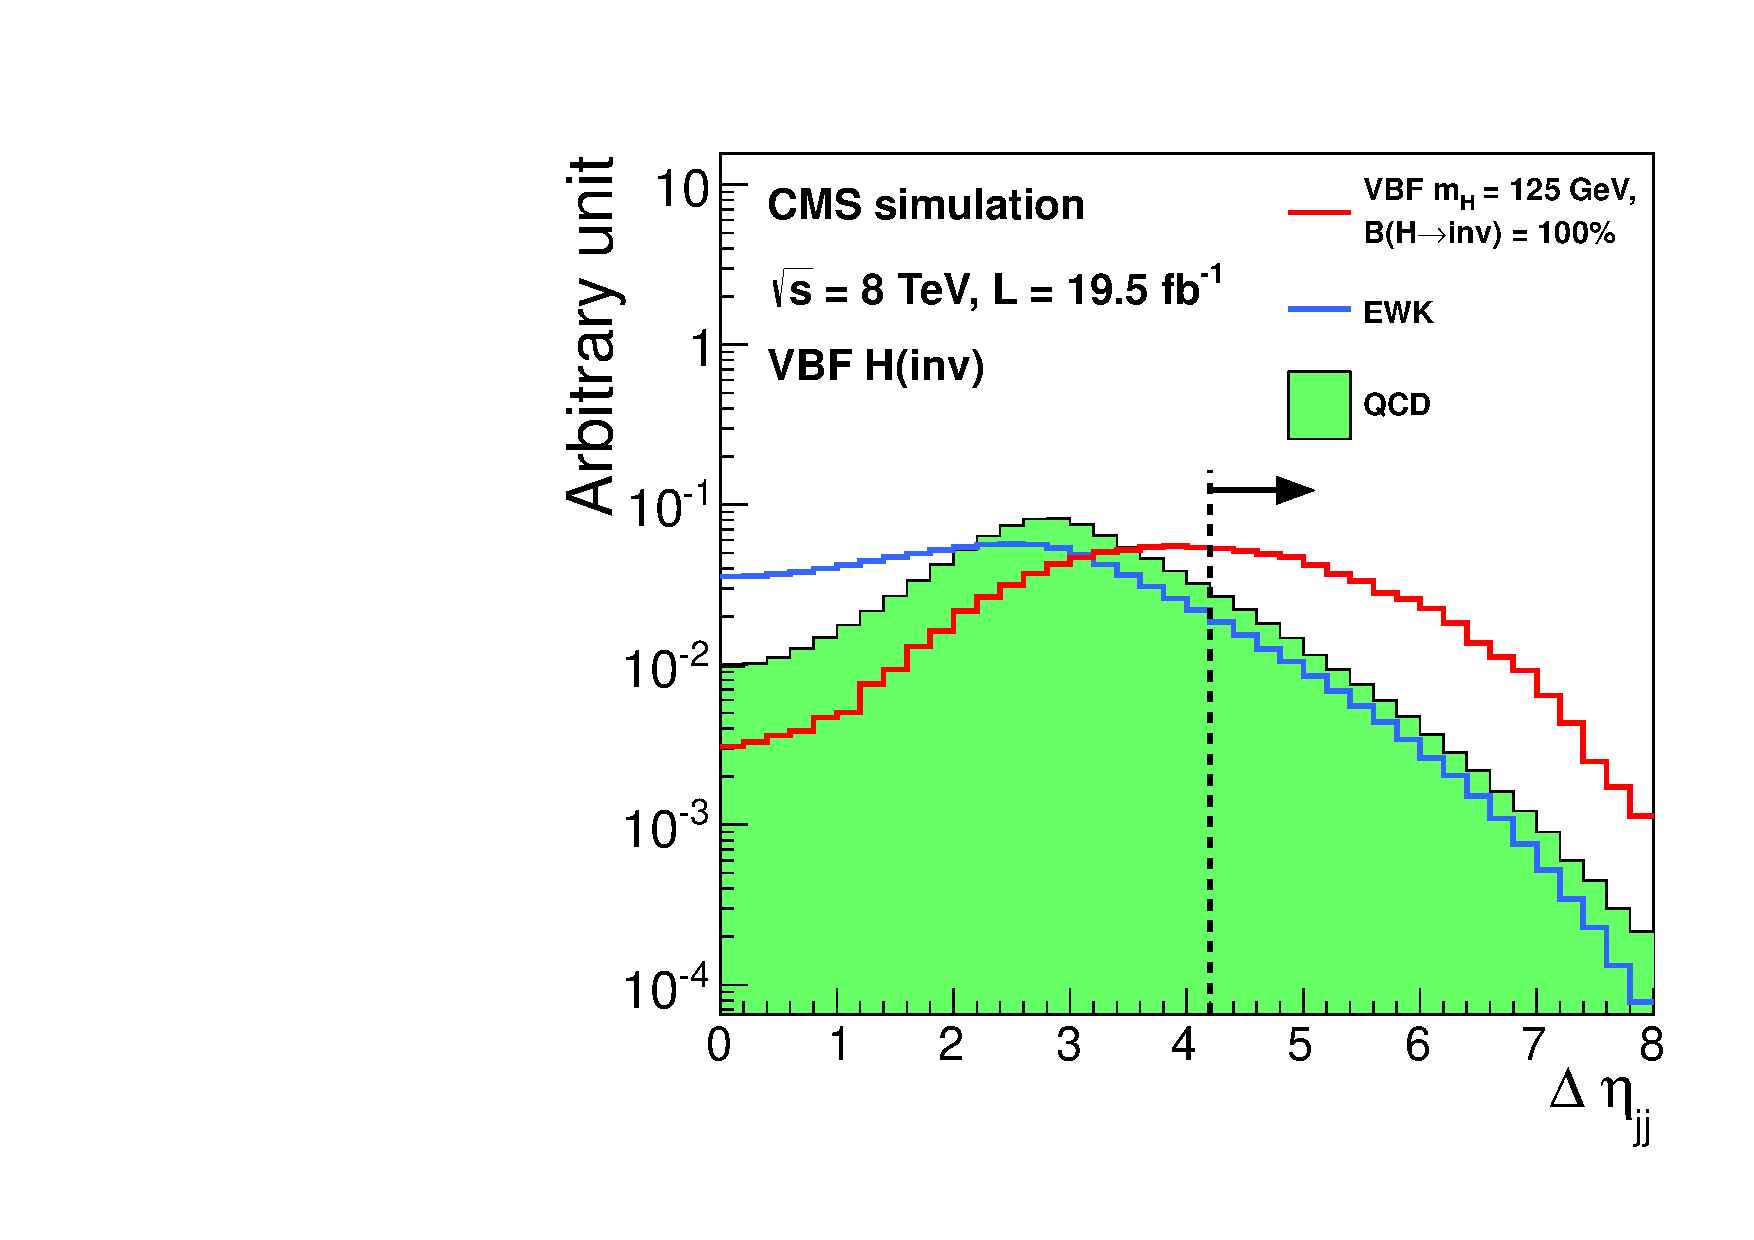
\includegraphics[width=.6\largefigwidth]{plots/prompt/VBF-Dijet-DEta.pdf}}

  \subfloat[]{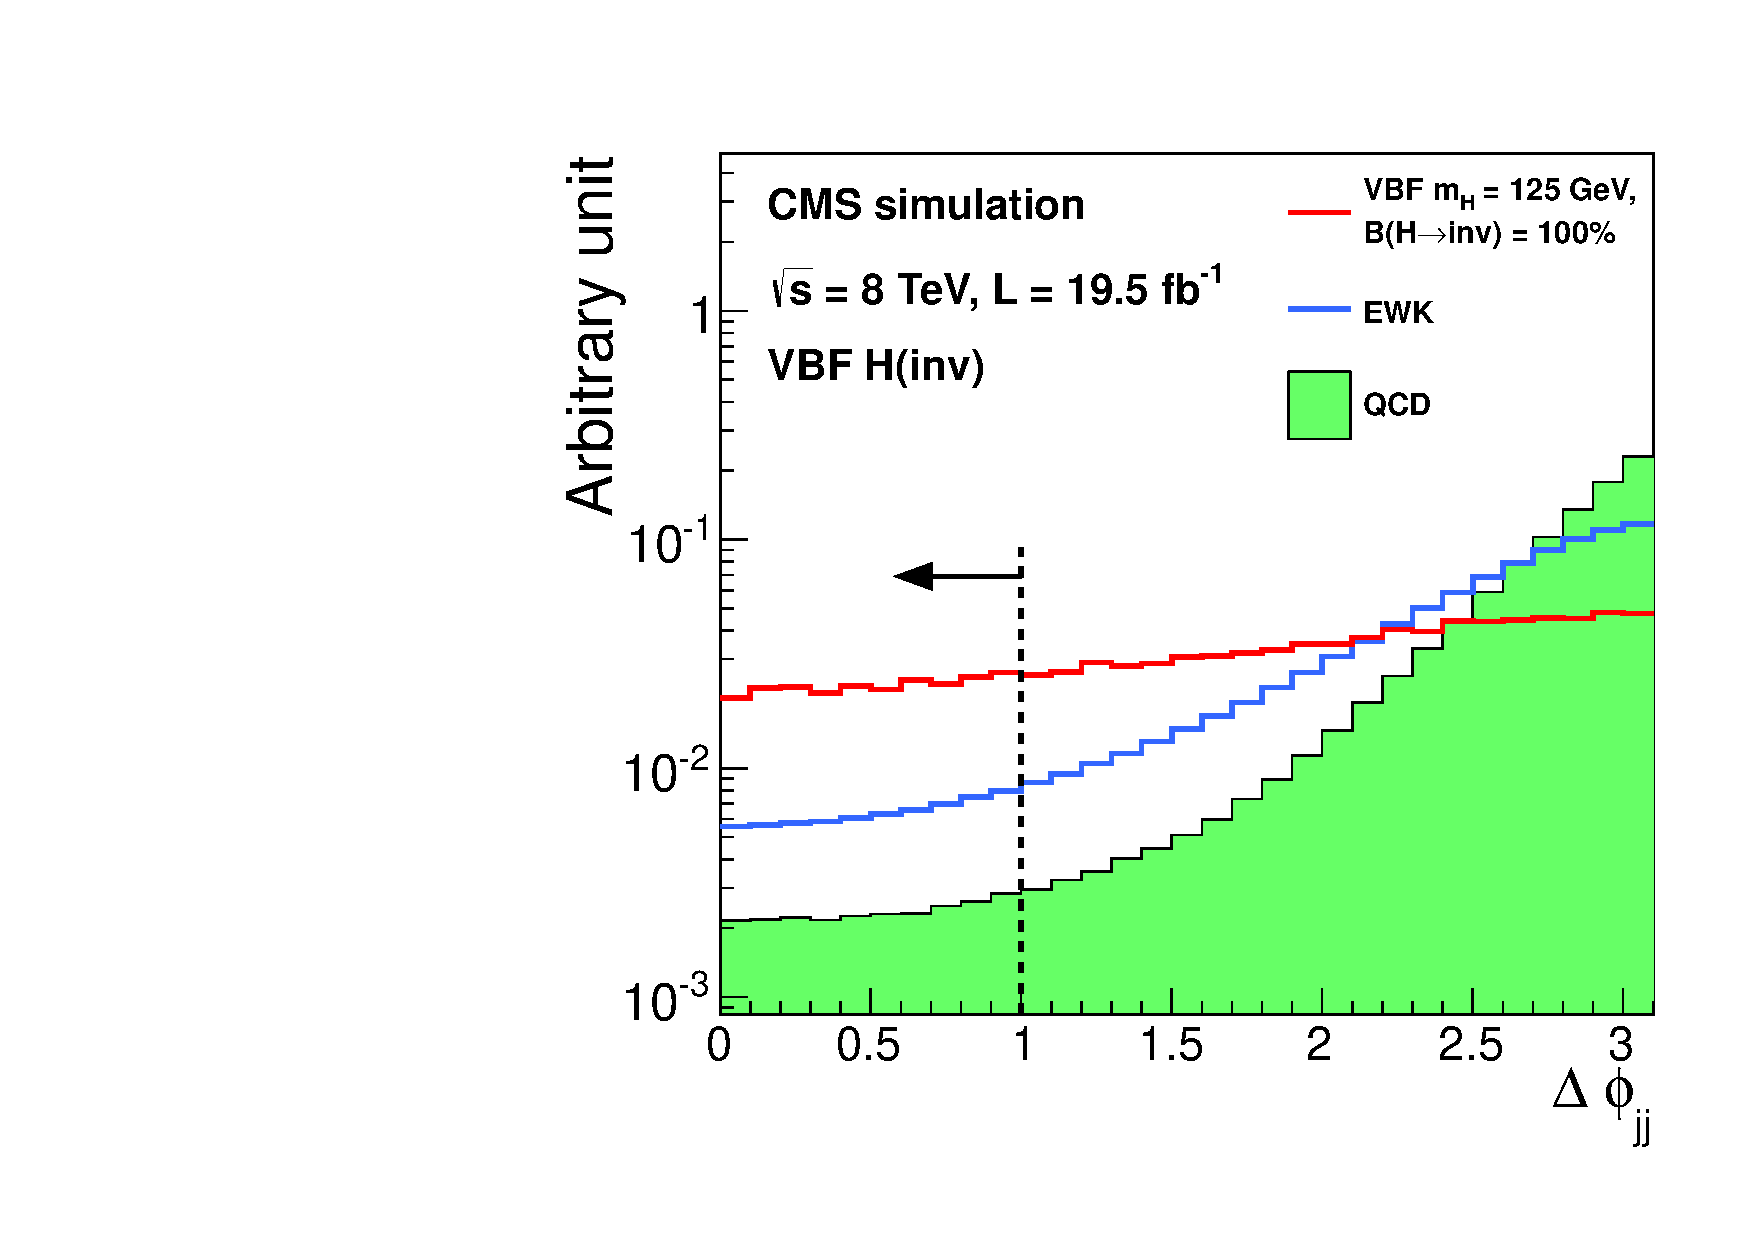
\includegraphics[width=.6\largefigwidth]{plots/prompt/VBF-Dijet-DPhi.pdf}}
  \subfloat[]{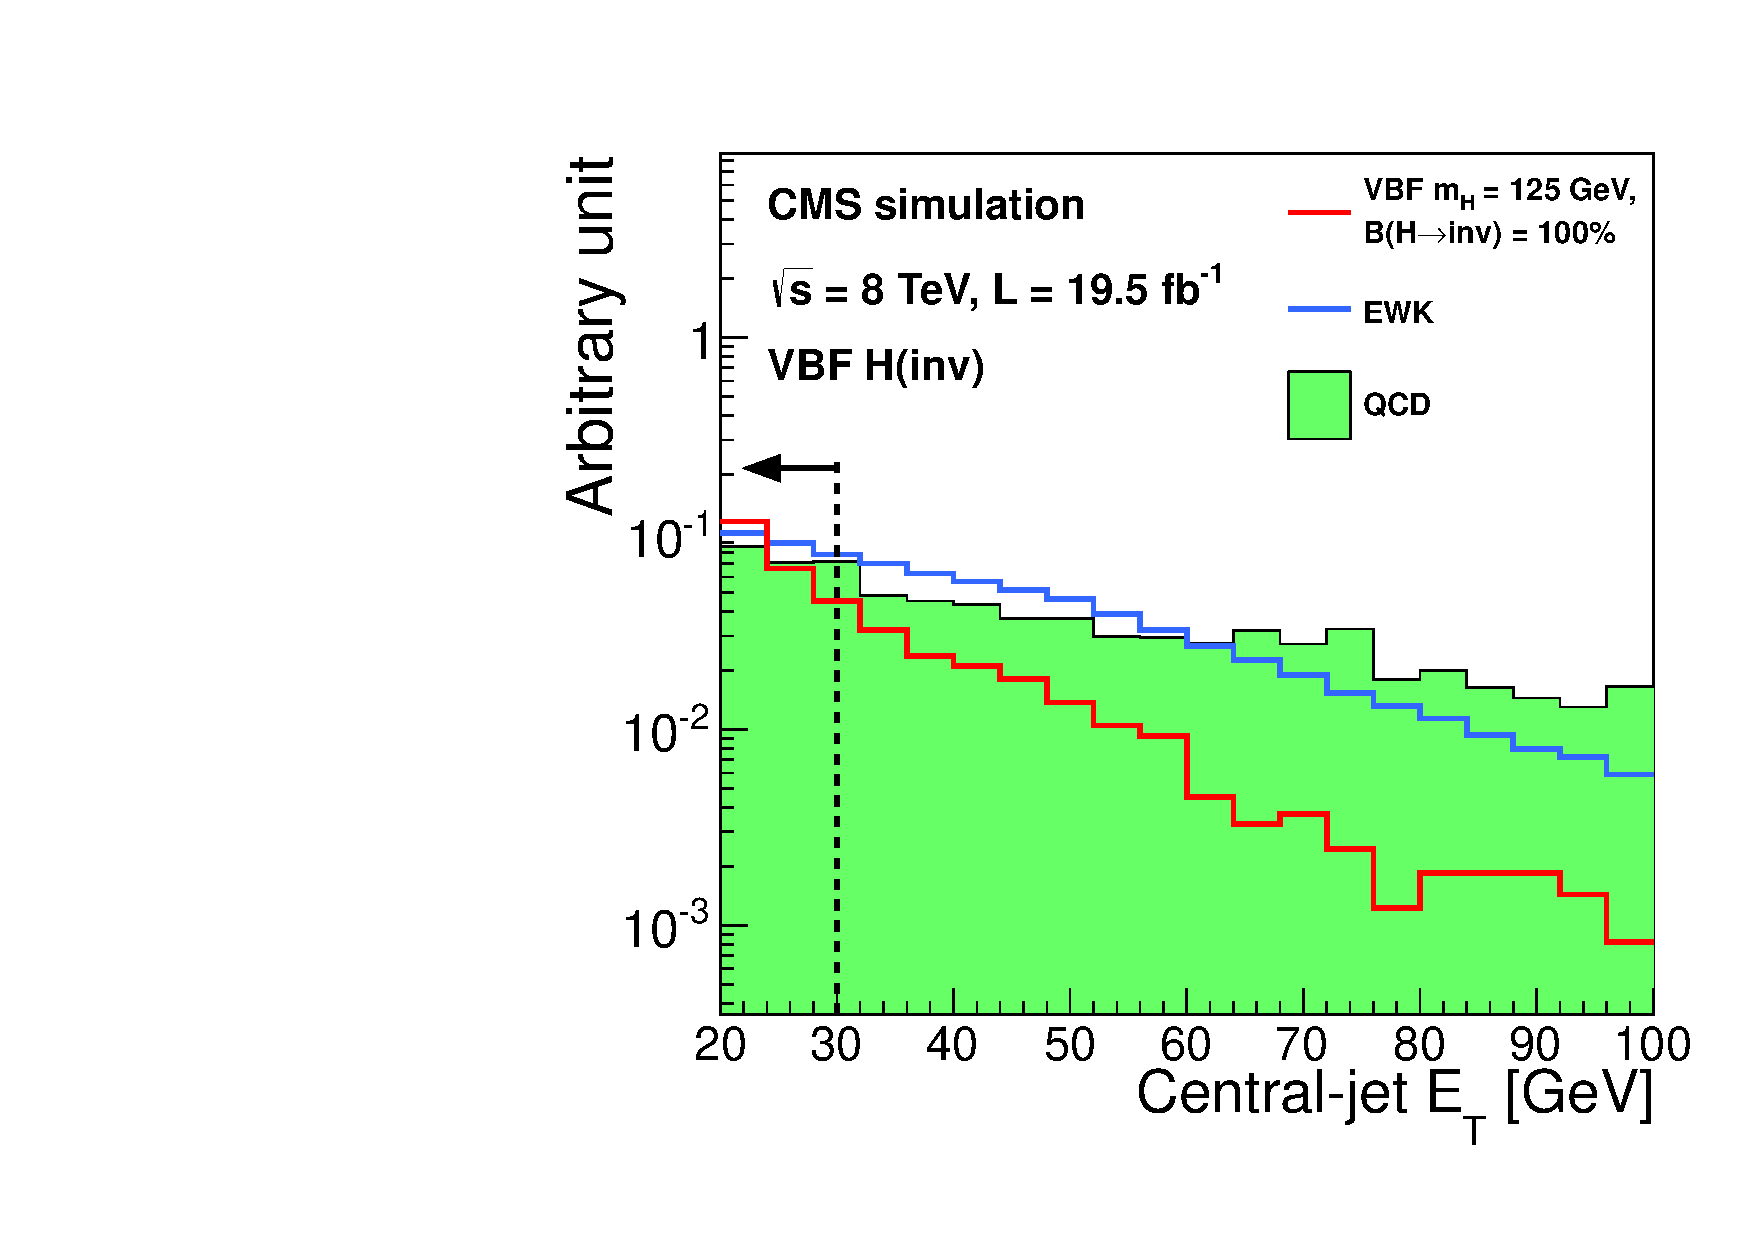
\includegraphics[width=.6\largefigwidth]{plots/prompt/VBF-CJV-pT.pdf}}
  \caption{Distributions of (a) $M_{jj}$, (b) $\Delta\eta_{jj}$, (c) $\Delta\phi_{jj}$ and (d) leading central jet \pt in background and signal \ac{MC} events. The events shown are required to have two jets in opposite forward/backward halves of the detector with \pt$>50$ \GeV, $|\eta|<4.7$, $M_{jj}>150$ \GeV and \MET$>130$ \GeV. The dashed lines indicate the offline selection criteria applied to these variables ~\cite{Chatrchyan:2014tja}.}
  \label{fig:promptcontrolplots}
\end{figure}


\section{Background estimation}%??
\label{sec:promptbkg}
As discussed in \SectionRef{sec:promptsel} there are several background processes which are capable of producing VBF-like jets in association with \MET. The analysis' event selection removes most of the events from these processes, however a significant number still remain and it is important to estimate this number precisely. Data-driven methods, where data ``control regions'', which are similar to the signal region, are used to estimate the most significant backgrounds. This data-driven approach is particularly important due to the very stringent kinematic requirements placed on the tag jets, which lead to high uncertainties on estimates taken from \ac{MC} alone. The particular method used to estimate each of the backgrounds will be described in this section.

\subsection{\PW$\rightarrow e\nu$ + jets}
\label{sec:promptwenu}
The ``$\PW$+jets'' background where the $\PW$ boson decays to an electron and an electron neutrino, $\PW\rightarrow e\nu$ is estimated using single electron events. All aspects of the event selection are the same as those used in the singal region, except for the electron veto, which is replaced with the requirement that there is exactly one tight electron, with $p_{T}>20$ \GeV, in the event and no other veto electrons. These requirements give a single electron control region with events with jets that have the same kinematics as those in the signal region, but which is dominated by $\PW$ boson decays to electrons.

The estimated number of $\PW\rightarrow e\nu$ events in the signal region is then estimated by using the ratio between the expected number of events in the signal and control regions from \ac{MC} to extrapolate from the number of events seen in data in the single electron control region using the following formula:
\begin{equation}
  \label{eq:wdatabkg}
  N^{S}_{Exp}=\left(N^{C}_{Data}-N^{C}_{Bkg}\right)\cdot\frac{N^{S}_{MC}}{N^{C}_{MC}},
\end{equation}
where $N^{S}_{Exp}$ is the number of expected events in the signal region from this background process, $N^{C}_{Data}$ is the number of events seen in the control region in data, $N^{C}_{Bkg}$ is the number of events from other backgrounds in the control region estimated using \ac{MC}, which is expected to be small, and $N^{S}_{MC}$ and $N^{C}_{MC}$ are the numbers of events predicted by \ac{MC} to be in the signal and control regions respectively. The fact that estimations from \ac{MC} are only used in ratios or where they are expected to be small removes any dependence of the final background estimation on the overall rate of the process predicted by \ac{MC}, and instead allows the observed rate in data to be used. It is important that the shape of the variables which differ between the control and signal regions are well modelled by the \ac{MC}. The modelling of the shape of two key variables, the \MET and the electron \pt, are shown in \FigureRef{fig:promptwenu}, where it can be seen that whilst the overall rate is significantly different between data and \ac{MC}, the shape of the distribution is modelled well.  The inputs and results of the background estimation are shown in \TableRef{tab:promptwenu}.

%tables from AN-13-205
\begin{table}
  \caption{The inputs and results of the $\PW\rightarrow e\nu$ background estimation. $N_{\PW\rightarrow e\nu}$ is in the signal region the number of events expected from $\PW\rightarrow e\nu$ backgrounds, and in the control region the number of events remaining in the region after the subtraction of other backgrounds.}
  \label{tab:promptwenu}
  \begin{tabular}{|l|c|c|}
    \hline
    & Signal region & Control region \\
    \hline
    $N_{Data}$ & N/A & 64\\
    $N_{Bkg}$ & N/A & $7.42\pm2.78$(\ac{MC} stat.) \\
    $N_{MC}$& $105\pm10$(\ac{MC} stat.) & $86.6\pm 7.1$(\ac{MC} stat.) \\
    $N_{\PW\rightarrow e\nu}$& $68.7\pm 10.3$(stat.)$\pm 8.8$(\ac{MC} stat.) & $56.6\pm 8.5$(stat.) \\
    \hline
  \end{tabular}
\end{table}

%plot from AN-12-403
\begin{figure}
  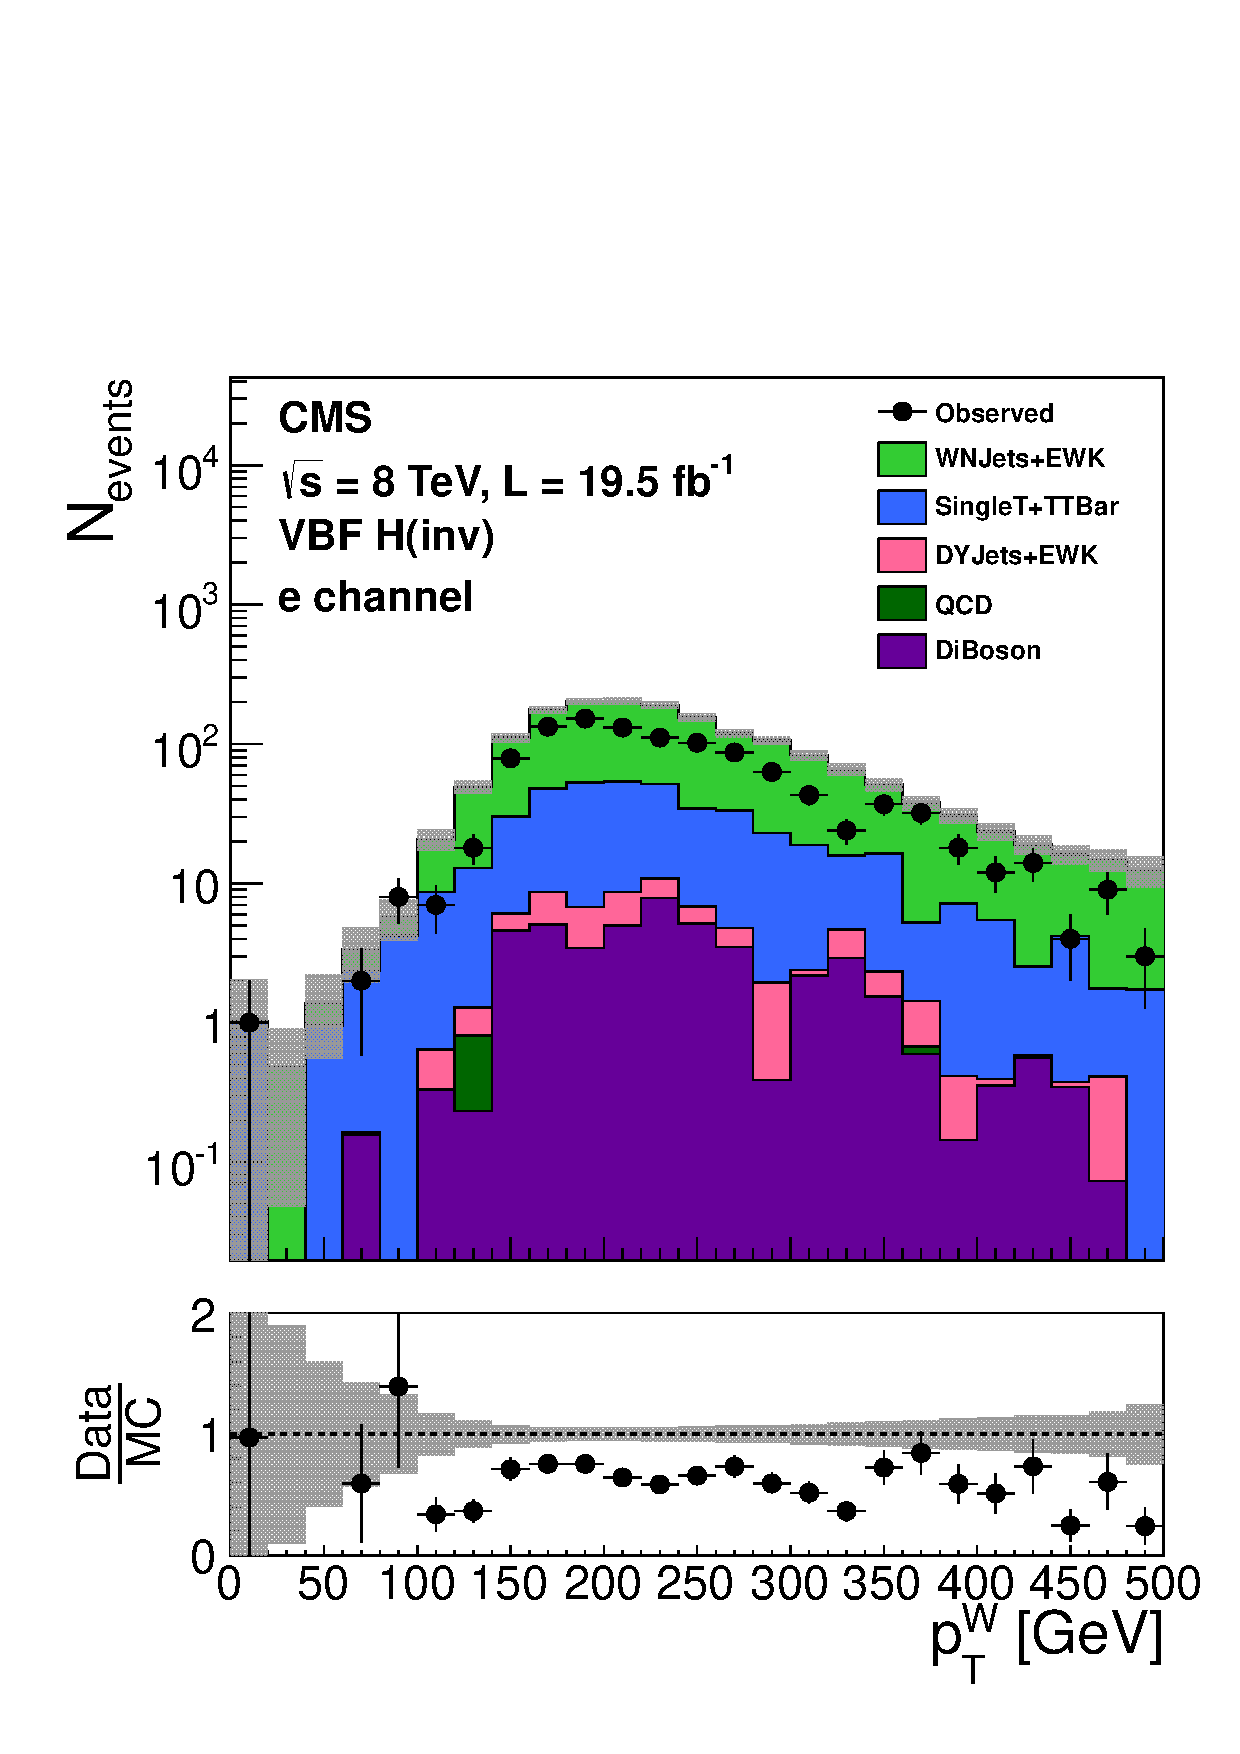
\includegraphics[width=.6\largefigwidth]{plots/prompt/AN-12-403-figs/hWEl_WpT.pdf}
  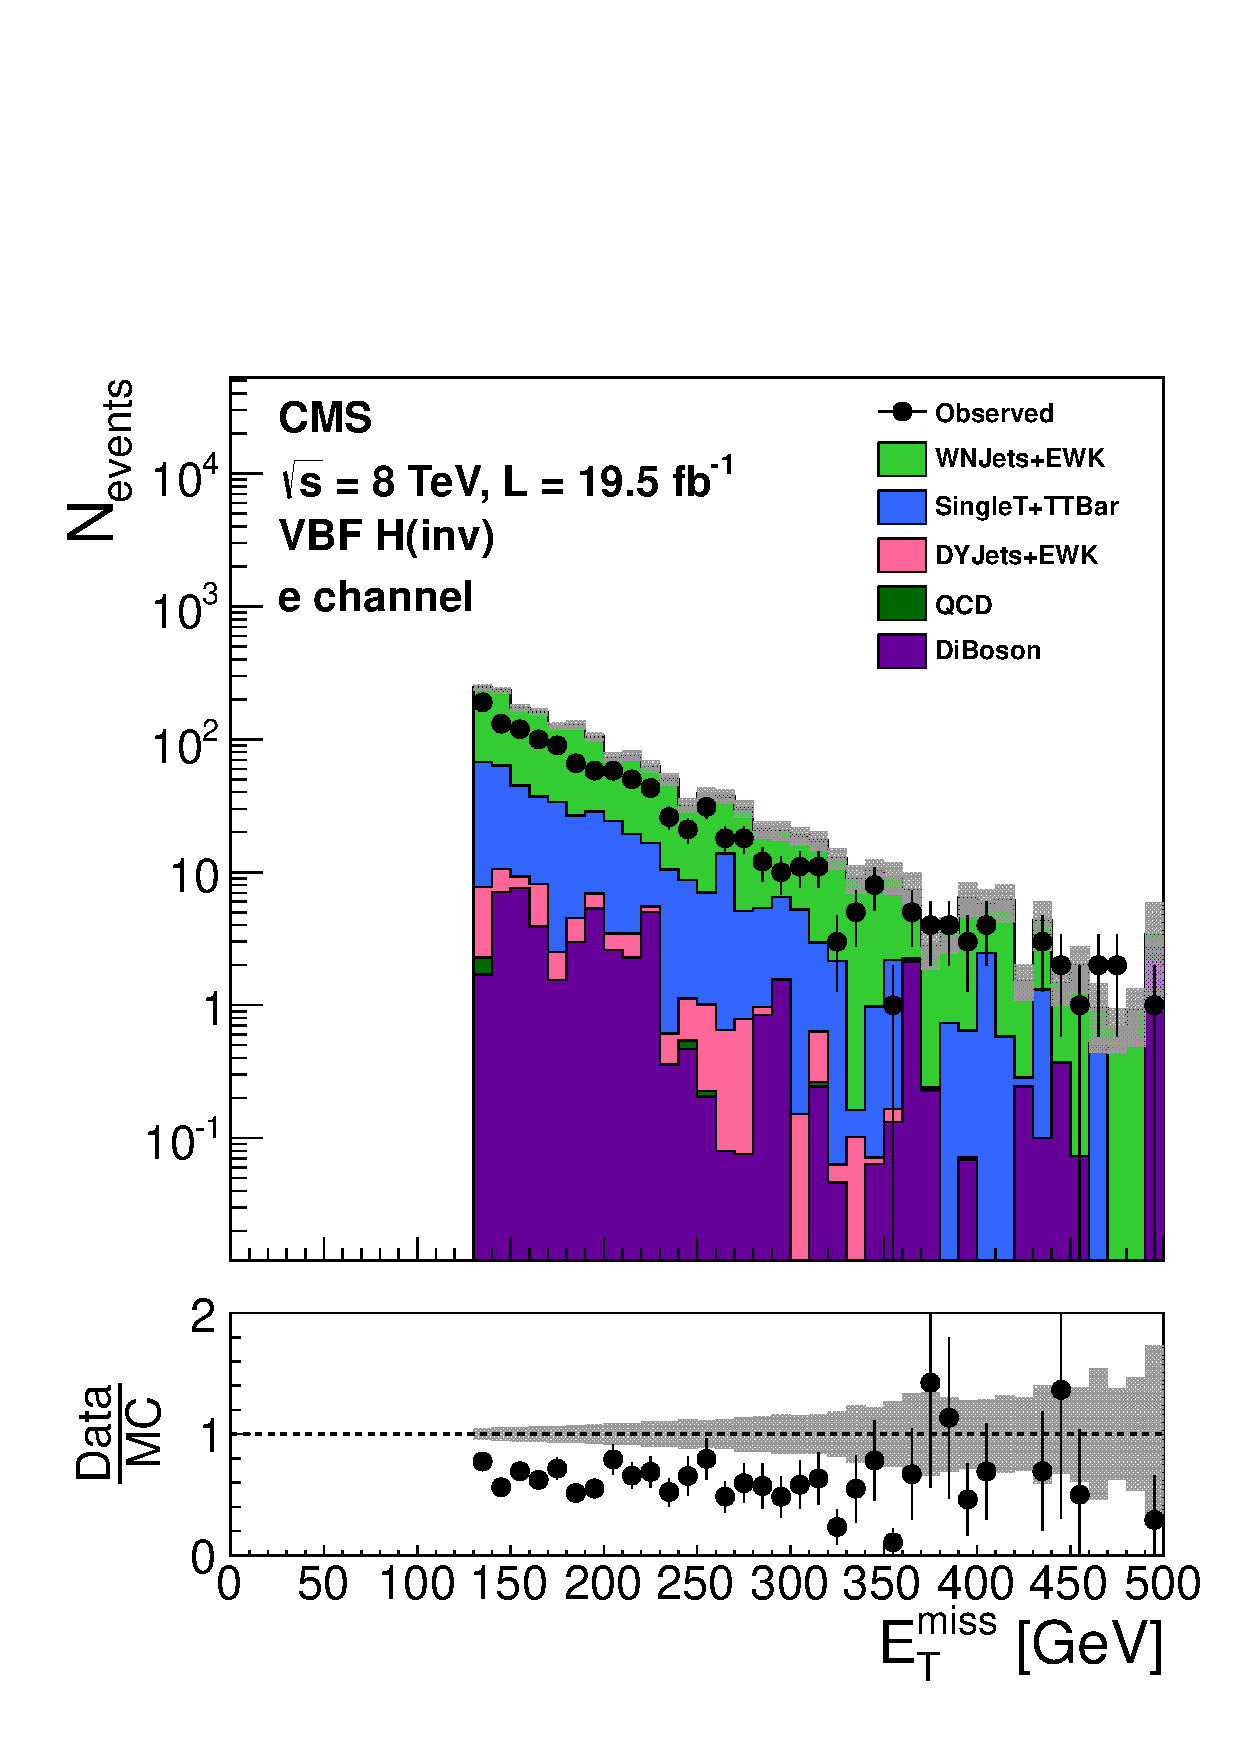
\includegraphics[width=.6\largefigwidth]{plots/prompt/AN-12-403-figs/hWEl_MET.pdf}
  \caption{Distributions of the visible $\PW$ boson \pt (i.e. the electron \pt) (left) and \MET (right) in the single electron control region. The hatched region illustrates the systematic uncertainty~\cite{ARTICLE:CMSAN-12-403}.}
  \label{fig:promptwenu}
\end{figure}

\subsection{\PW$\rightarrow \mu\nu$ + jets}
\label{sec:promptwmunu}
The method used to estimate the background from $\PW$+jets where the $\PW$ boson decays to a muon and a muon neutrino, $\PW\rightarrow\mu\nu$, is very similar to that used for $\PW\rightarrow e\nu$. A single muon control region is used, again with identical selection to the signal region except for the modification of the lepton veto, in this case by replacing the muon veto with the requirement that there is exactly one tight muon, with \pt$>20$ \GeV, and no other veto muons. \EquationRef{eq:wdatabkg} is then used, with the control region now being the single muon control region, to estimate the number of events from $W\rightarrow\mu\nu$ expected in the signal region. The inputs and results of the background estimation are shown in \TableRef{tab:promptwmunu}, and distributions of the muon \pt and the \MET in the single muon control region are shown in \FigureRef{fig:promptwmunu}.

%tables from AN-13-205
\begin{table}
  \caption{The inputs and results of the $\PW\rightarrow \mu\nu$ background estimation. $N_{\PW\rightarrow \mu\nu}$ is in the signal region the number of events expected from $\PW\rightarrow \mu\nu$ backgrounds, and in the control region the number of events remaining in the region after the subtraction of other backgrounds.}
  \label{tab:promptwmunu}
  \begin{tabular}{|l|c|c|}
    \hline
    & Signal region & Control region \\
    \hline
    $N_{Data}$ & N/A & 216\\
    $N_{Bkg}$ & N/A & $30.1\pm 4.5$(\ac{MC} stat.) \\
    $N_{MC}$& $108\pm 10$(\ac{MC} stat.) & $306\pm 15$(\ac{MC} stat.) \\
    $N_{\PW\rightarrow \mu\nu}$& $65.8\pm 5.4$(stat.)$\pm 6.7$(\ac{MC} stat.) & $186\pm 15$(stat.) \\
    \hline
  \end{tabular}
\end{table}

%plot from AN-12-403
\begin{figure}
  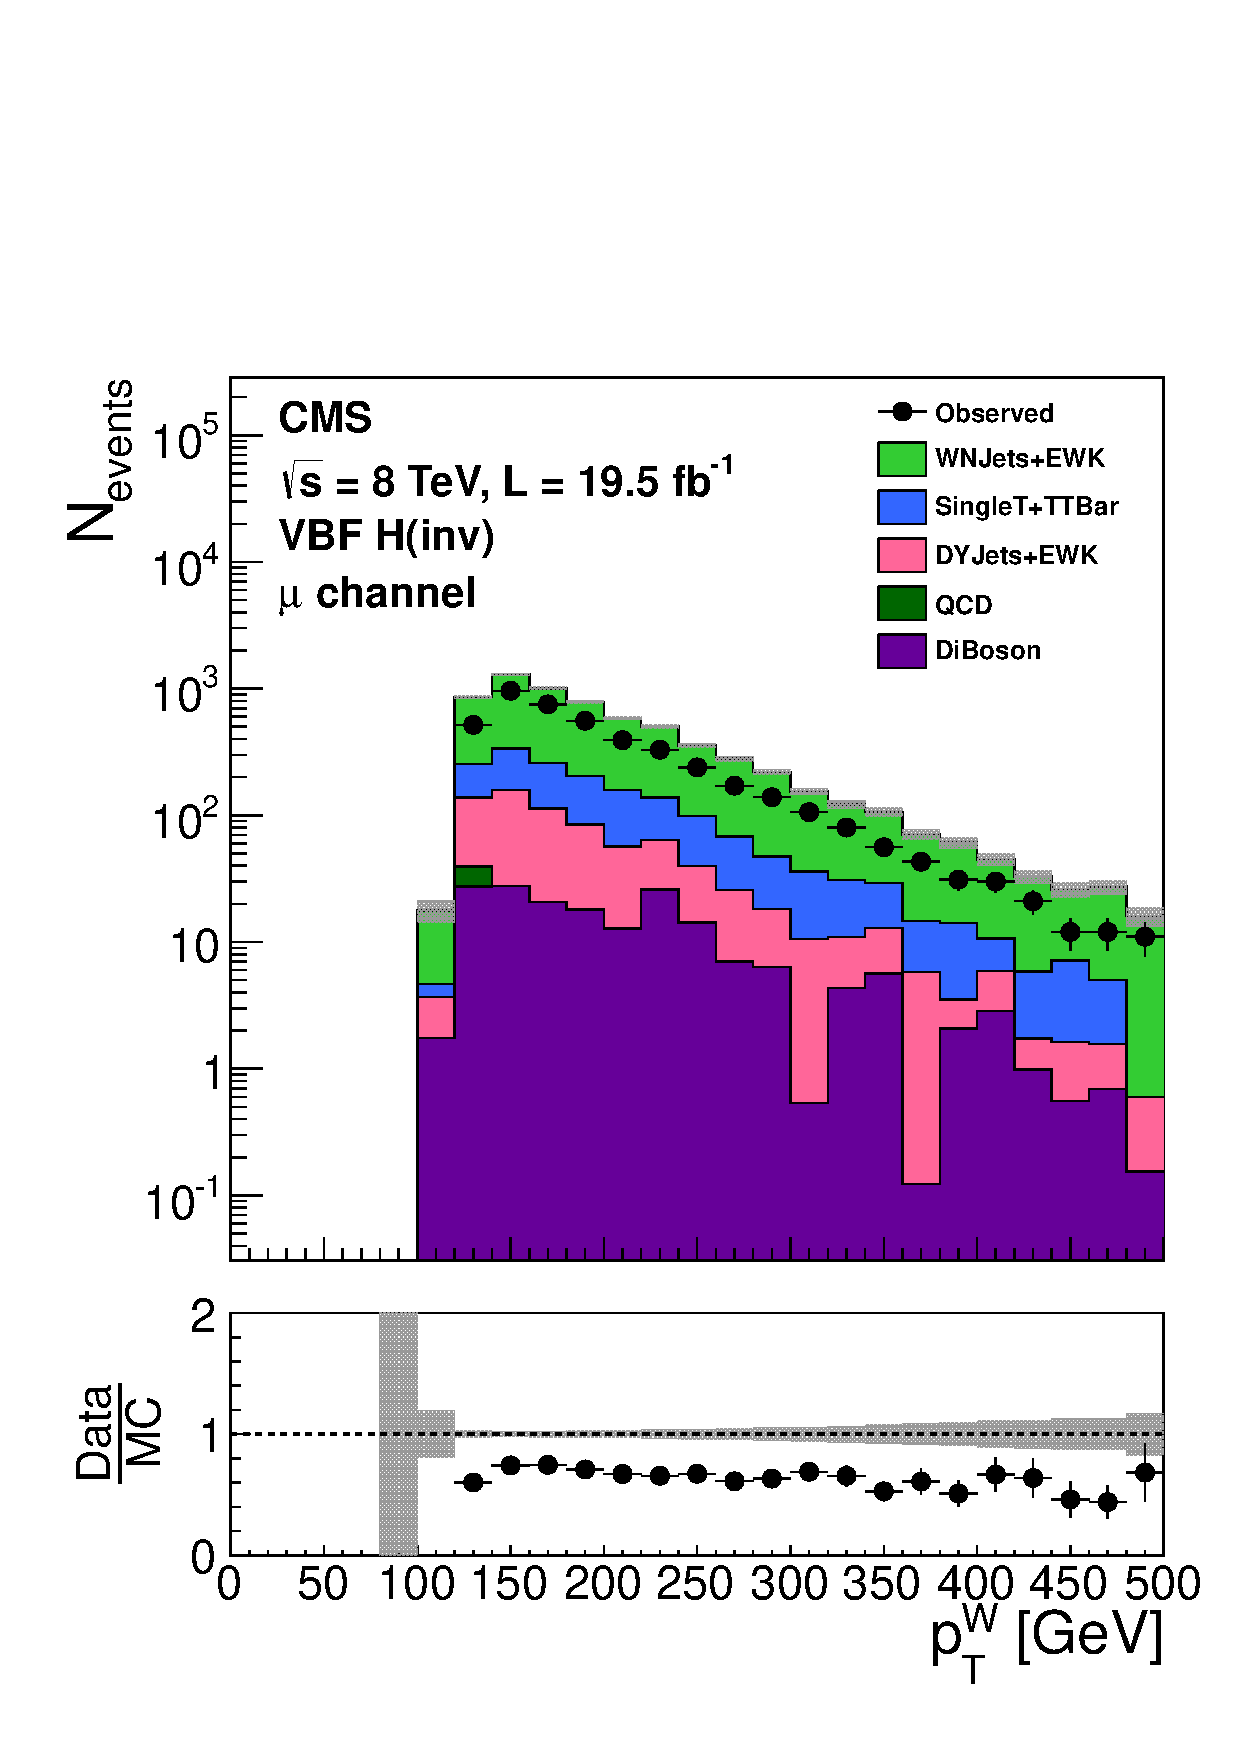
\includegraphics[width=.6\largefigwidth]{plots/prompt/AN-12-403-figs/hWMu_WpT.pdf}
  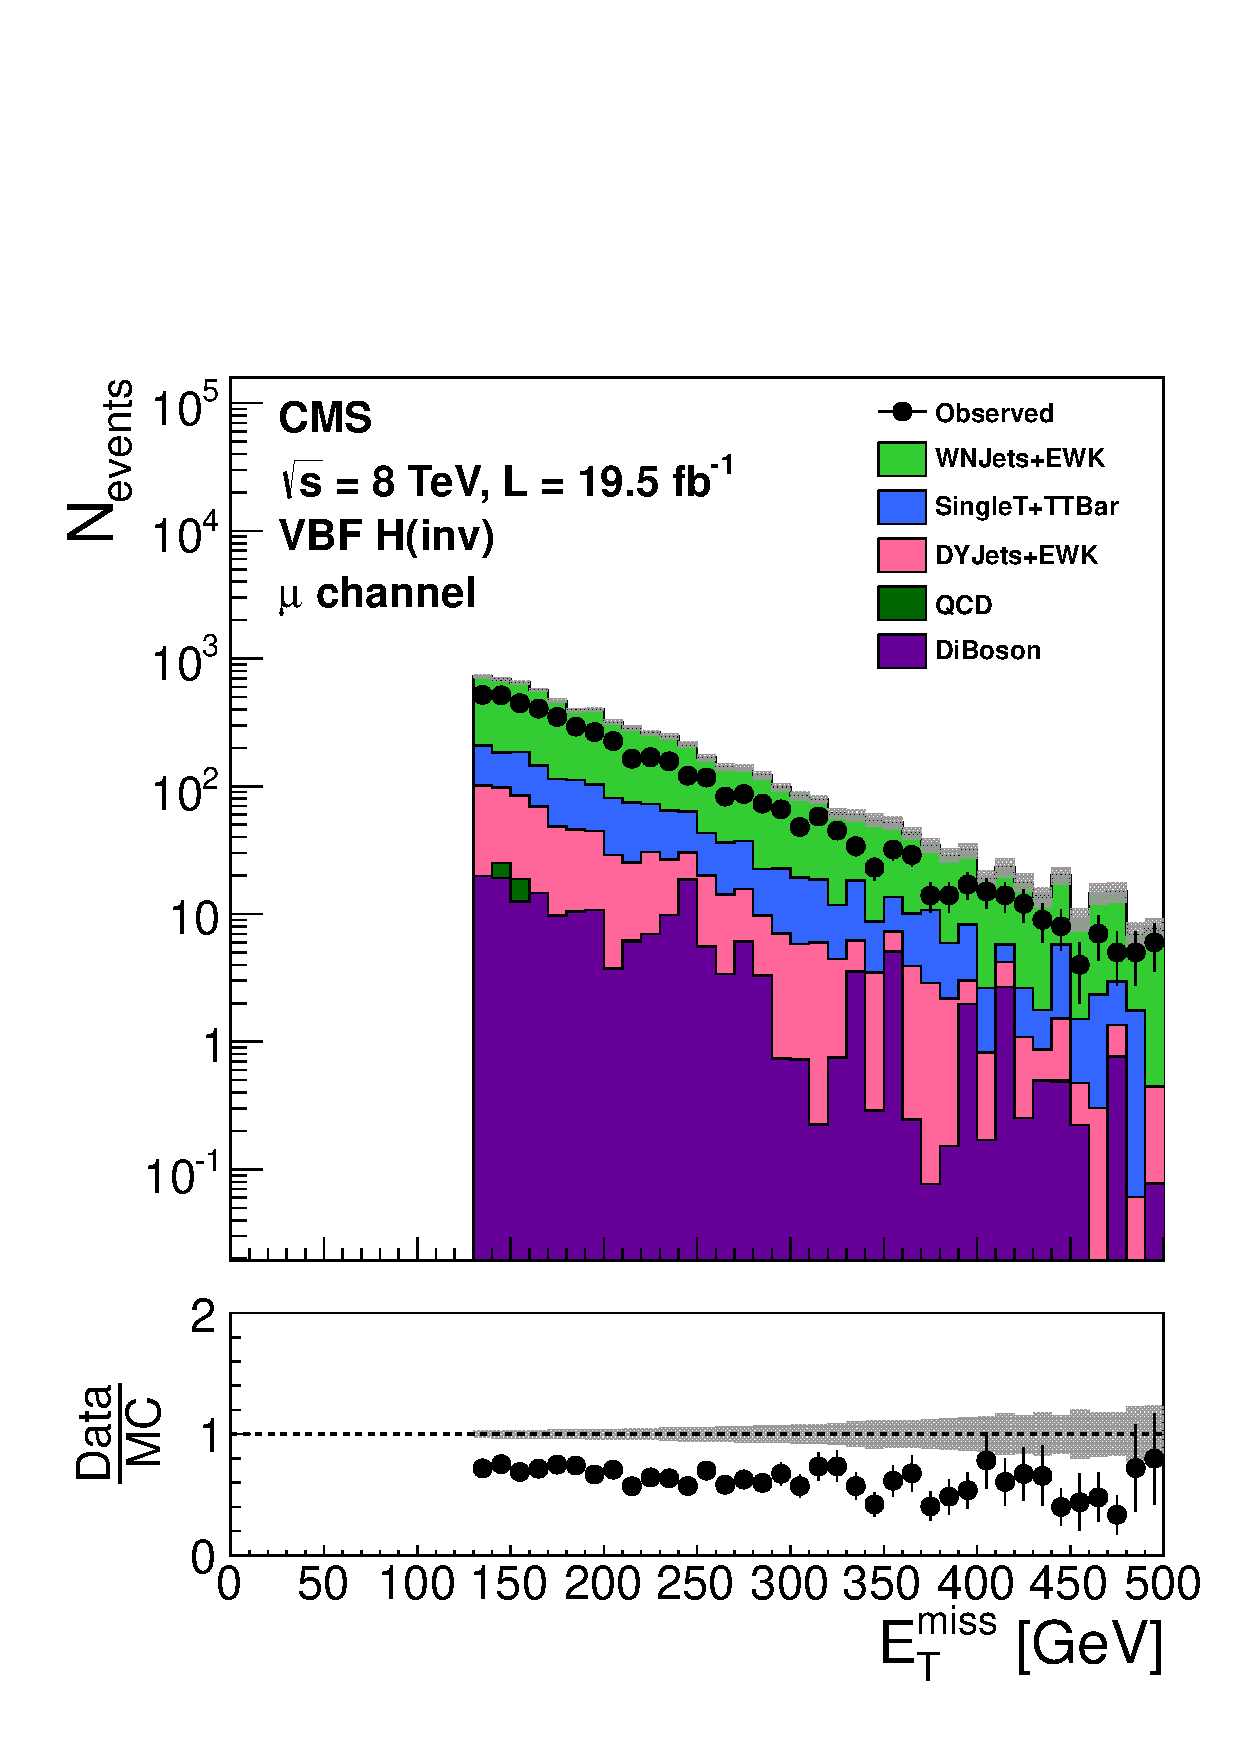
\includegraphics[width=.6\largefigwidth]{plots/prompt/AN-12-403-figs/hWMu_MET.pdf}
  \caption{Distributions of the visible $\PW$ boson \pt (i.e. the muon \pt) (left) and \MET (right) in the single muon control region. The hatched region illustrates the systematic uncertainty~\cite{ARTICLE:CMSAN-12-403}.}
  \label{fig:promptwmunu}
\end{figure}

\subsection{\PW$\rightarrow \tau\nu$ + jets}
\label{sec:promptwtaunu}
The background from $\PW$+jets where the $\PW$ boson decays to a tau and a tau neutrino, $\PW\rightarrow\tau\nu$, is estimated using a single tau control region data-driven method. However, in this case the control region used has more differences from the signal region than those used above. The reason for these increased differences is that the reconstruction efficiency for tau leptons is significantly lower than that for electrons or muons, and they are also more likely to be misreconstructed as jets, causing the event to be vetoed by the \ac{CJV}. Altering the signal region by adding a requirement that there is exactly one tau with \pt$>20$ \GeV\, results in a region with only $3.76\pm 1.27$(stat.) \PW+jets events expected. In order to increase the number of events in the single tau control region as well as adding the tau requirement, the \ac{CJV} is also removed. The resulting control region has $29.2\pm 3.61$(stat.) \PW+jets events expected and thus a much lower statistical uncertainty.

The single tau control region has the same requirements as the signal region except that a requirement that there is exactly one tau with \pt$>20$ \GeV\, is added, and the \ac{CJV} is removed to increase the number of events in the control region, and thus reduce the statistical error on the estimation of this background. As there is no veto of tau leptons in the signal region the tau control region and the signal region are not mutually exclusive. However, as stated above the number of events in the signal region with identified taus is expected to be small, so the overlap is considered negligible.

%cross-check of tau discriminant https://indico.cern.ch/event/259915/session/1/contribution/2/attachments/458506/635408/tauid090713.pdf
In addition to the tau identification algorithm described in \SectionRef{sec:taus}, alternative algorithms were studied to check for better performance in terms of identification efficiency and fake rate. Specifically an alternative isolation algorithm was investigated which used an \ac{MVA} approach to estimate the isolation sum, as well as different working points for the anti-electron and anti-muon discriminators. The tau identification efficiency was found to be higher for both the alternative isolation algorithm and different working points for the anti-lepton discriminators, being twice as large if both were used compared to the standard tau identification. However, the rate of $\PW\rightarrow e\nu$ events being identified as $\PW\rightarrow\tau\nu$ was also significantly increased, going from 2\$ for the standard identification to 15\% where the alternative isolation and anti-lepton discriminators were used. It was therefore decided to use the tau identification described in \SectionRef{sec:taus}.

The final estimation of the background from $W\rightarrow\tau\nu$ is carried out using \EquationRef{eq:wdatabkg}, with the single tau control region with no \ac{CJV} being used as the control region. The inputs and results of the background estimation are shown in \TableRef{tab:promptwtaunu}, and distributions of the tau \pt and $\Delta\phi_{jj}$ in the single tau control region are shown in \FigureRef{fig:promptwtaunu}.

%tables from AN-13-205
\begin{table}
  \caption{The inputs and results of the $\PW\rightarrow \tau\nu$ background estimation. $N_{\PW\rightarrow \tau\nu}$ is in the signal region the number of events expected from $\PW\rightarrow \tau\nu$ backgrounds, and in the control region the number of events remaining in the region after the subtraction of other backgrounds.}
  \label{tab:promptwtaunu}
  \begin{tabular}{|l|c|c|}
    \hline
    & Signal region & Control region \\
    \hline
    $N_{Data}$ & N/A & 32\\
    $N_{Bkg}$ & N/A & $14.7\pm 3.4$(\ac{MC} stat.) \\
    $N_{MC}$& $95.6\pm 8.5$(\ac{MC} stat.) & $29.2\pm 3.6$(\ac{MC} stat.) \\
    $N_{\PW\rightarrow \tau\nu}$& $56.5\pm 21.5$(stat.)$\pm 8.6$(\ac{MC} stat.) & $17.3\pm 3.9 $(stat.) \\
    \hline
  \end{tabular}
\end{table}

%plot from AN-12-403
\begin{figure}
  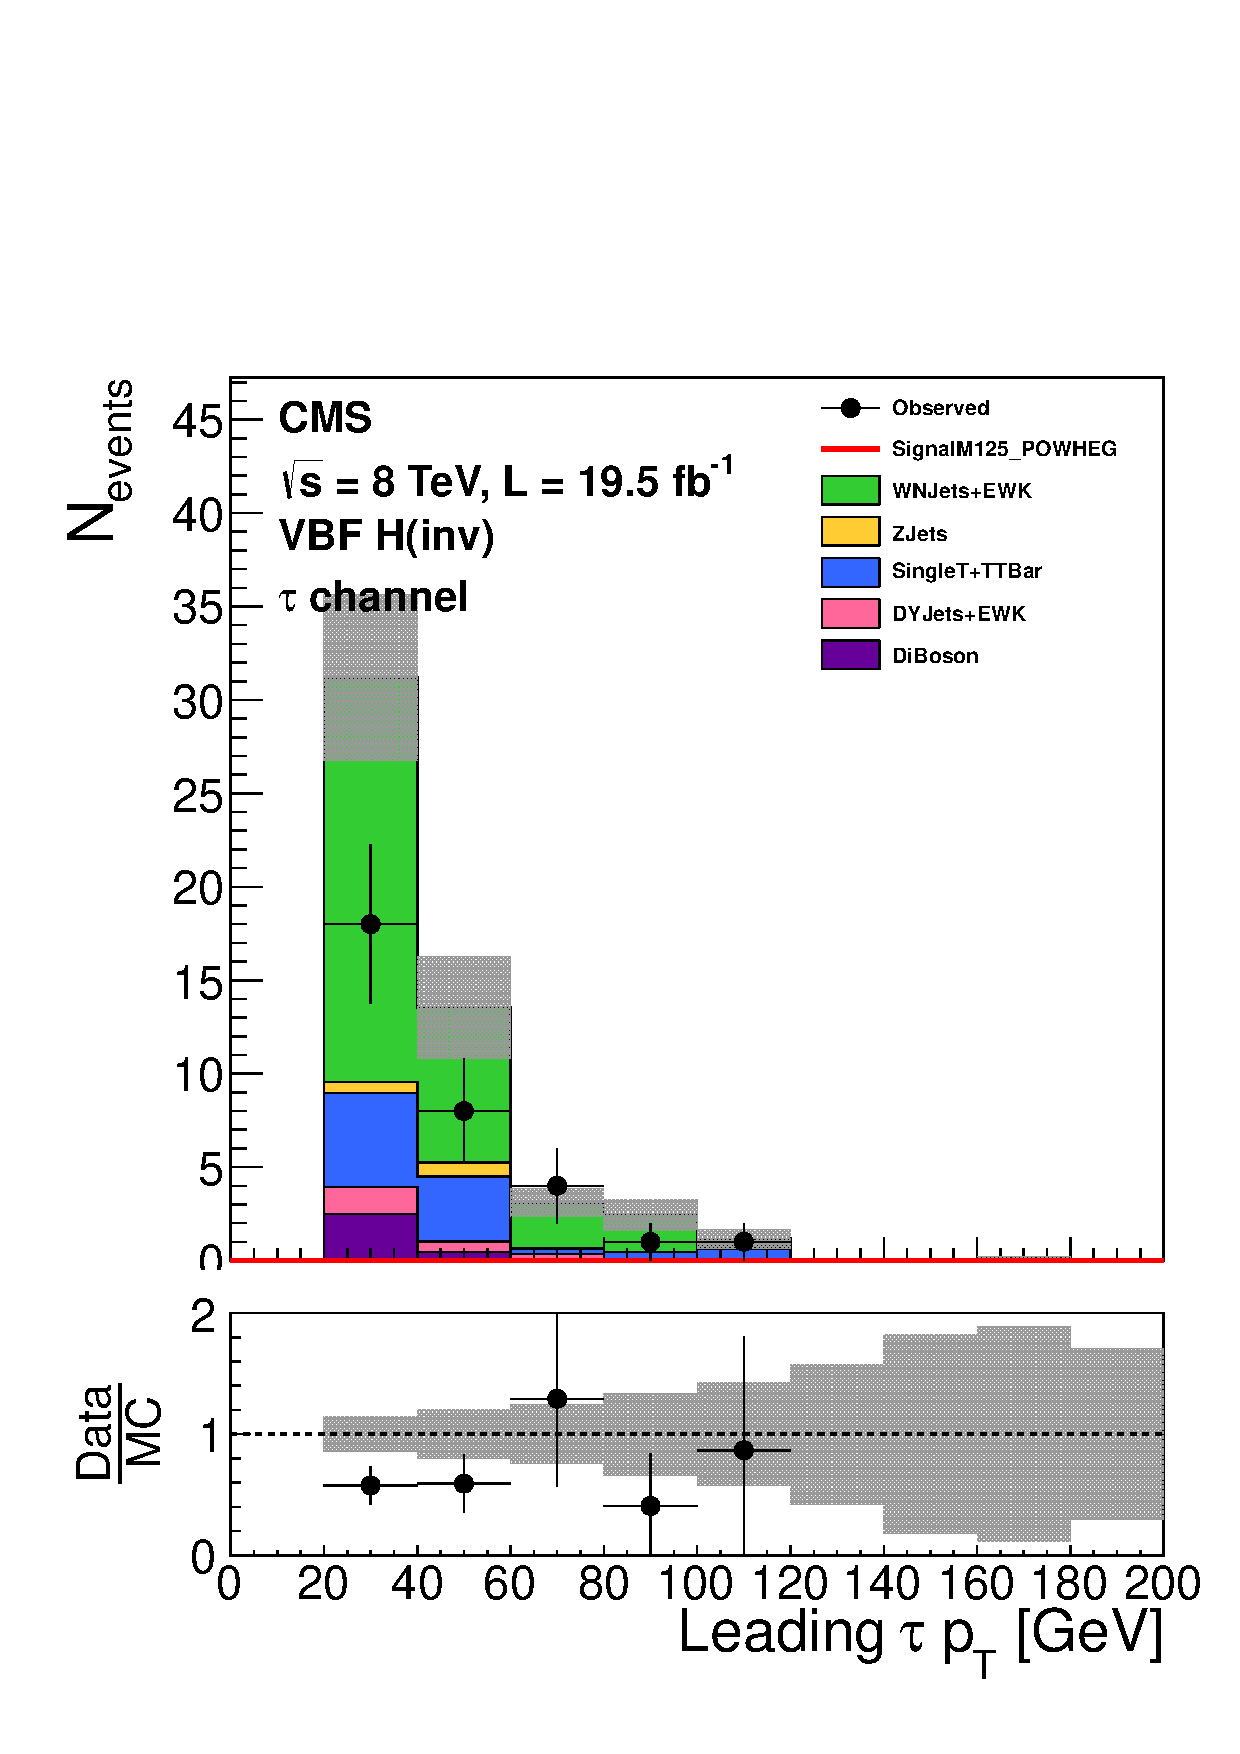
\includegraphics[width=.6\largefigwidth]{plots/prompt/AN-12-403-figs/hWTau_tau1Pt.pdf}
  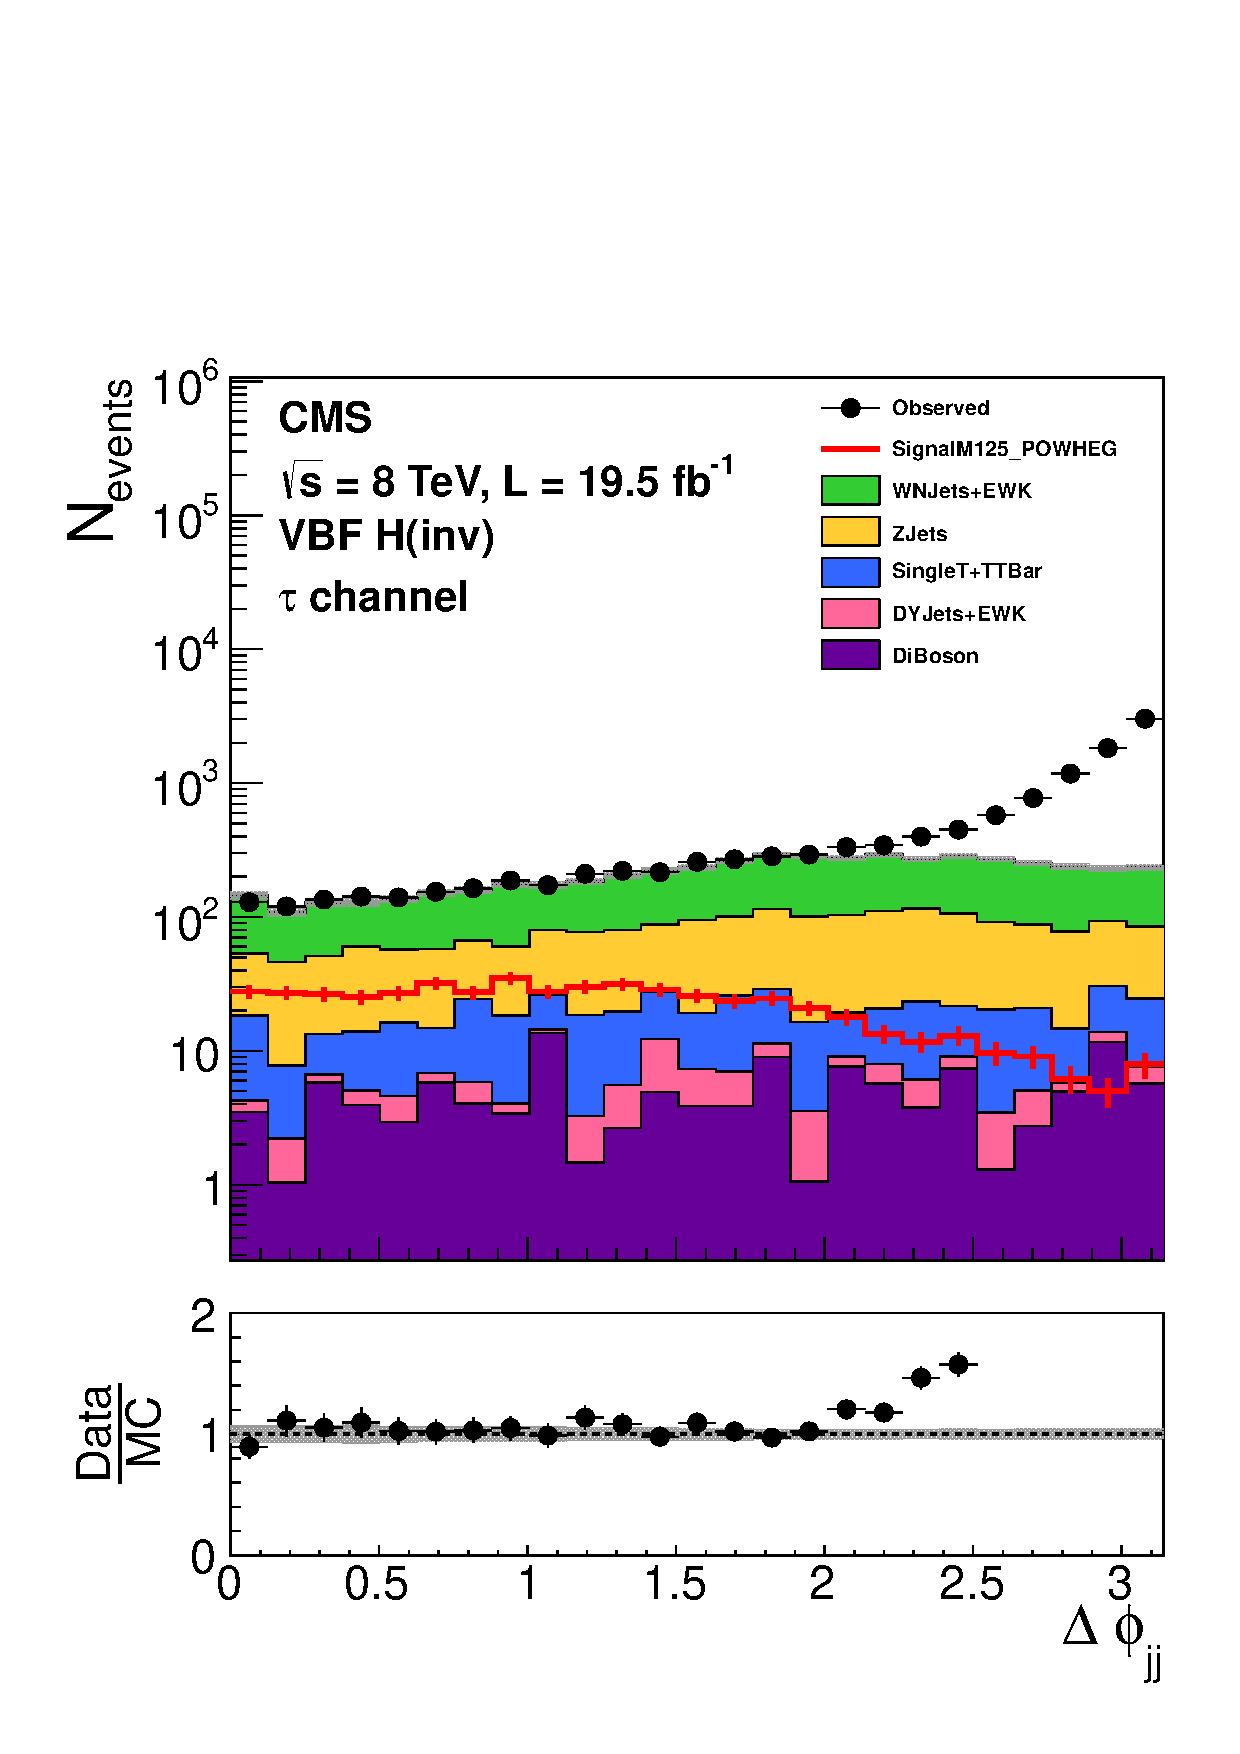
\includegraphics[width=.6\largefigwidth]{plots/prompt/AN-12-403-figs/hWTau_dPhiJJ.pdf}
  \caption{Distributions of the the tau \pt (left) and $\Delta\phi_{jj}$ (right) in the single tau control region. The hatched region illustrates the systematic uncertainty~\cite{ARTICLE:CMSAN-12-403}.}
  \label{fig:promptwtaunu}
\end{figure}

\subsection{\PZ$\rightarrow \nu\nu$ + jets}
\label{sec:promptznunu}
The background from \PZ+jets where the \PZ decays to neutrinos, $\PZ\rightarrow\nu\nu$, is different from the \PW+jets backgrounds described above, in that nothing is required to be misidentified in order for these events to contribute to the signal region. The method used to estimate the $\PZ\rightarrow\nu\nu$ background therefore differs slightly from that used above. The method uses a dimuon control region which selects events from the process $\PZ/\gamma^{*}\rightarrow\mu\mu$. Due to this process being able to be mediated by a photon, the kinematics of the jets in $\PZ/\gamma^{*}\rightarrow\mu\mu$ events can be different to those from $\PZ\rightarrow\nu\nu$. The dimuon control region that is defined therefore has a requirement that the invariant mass of the dimuons be between 60 and 120 \GeV\,. The control region is otherwise identical to the signal region, except that the muon veto is replaced with a requirement that there are exactly two tight muons with \pt$>20$\GeV\, and no other veto muons.

As well as the possibility of different kinematics, $\PZ/\gamma^{*}\rightarrow\mu\mu$ and $\PZ/rightarrow\nu\nu$ also have different cross-sections. The formula used to estimate the $\PZ/\rightarrow\nu\nu$ background takes this into account as follows:
\begin{equation}
  \label{eq:zdatabkg}
  N^{S}_{Exp}=N^{C}_{Data}-N^{C}_{Bkg}\cdot\frac{\sigma\left(\PZ\rightarrow\nu\nu\right)}{\sigma\left(\PZ/\gamma^{*}\rightarrow\mu\mu\right)}\cdot\frac{\epsilon^{S}_{VBF}}{\epsilon^{C}_{VBF}},
\end{equation}
where $\sigma\left(\PZ\rightarrow\nu\nu\right)$ is the cross-section for $\PZ\rightarrow\nu\nu$ and $\sigma\left(\PZ/\gamma^{*}\rightarrow\mu\mu\right)$ is the cross-section for $\PZ/\gamma^{*}\rightarrow\mu\mu$. $\epsilon^{S}_{VBF}$ and $\epsilon^{C}_{VBF}$ are the efficiencies for $Z\rightarrow\nu\nu$ events to pass the signal region selection and $Z/\gamma^{*}\rightarrow\mu\mu$ events to pass the control region selection respectively. As Z bosons can be created via either \ac{QCD} or electroweak processes, which both have different cross-sections and efficiencies $\epsilon^{S}_{VBF}$ and $\epsilon^{C}_{VBF}$ are a cross-section weighted average of the efficiency for both types of production, calculated as:
\begin{align}
  \label{eq:zdataeffs}
  \epsilon^{S}_{VBF}&=\frac{ \sigma\left(\PZ\rightarrow\nu\nu,EWK\right) \frac{N^{S}_{MC}\left(EWK\right)} {N_{gen}\left(\PZ \rm{mass},EWK\right)} + \sigma\left(\PZ\rightarrow\nu\nu,QCD\right) \frac{N^{S}_{MC}\left(QCD\right)} {N_{gen}\left(\PZ \rm{mass},QCD\right)} } {\sigma\left(\PZ\rightarrow\nu\nu,EWK\right) + \sigma\left(\PZ\rightarrow\nu\nu,QCD\right)},\\
  \label{eq:zdataeffc}
  \epsilon^{C}_{VBF}&=\frac{  \sigma\left(\PZ/\gamma^{*}\rightarrow\mu\mu,EWK\right) \frac{N^{C}_{MC}\left(EWK\right)} {N_{gen}\left(EWK\right)} + \sigma\left(\PZ/\gamma^{*}\rightarrow\mu\mu,QCD\right) \frac{N^{S}_{MC}\left(QCD\right)} {N_{gen}\left(QCD\right)}  }{\sigma\left(\PZ/\gamma^{*}\rightarrow\mu\mu,EWK\right)+\sigma\left(\PZ/\gamma^{*}\rightarrow\mu\mu,QCD\right)}.
\end{align}
Where $EWK$ and $QCD$ donate where cross-sections or numbers of events are for electroweak or \ac{QCD} production of a $\PZ$ boson. $N_{gen}$ is the number of events in the Z+jets \ac{MC} sample at generator level. Due to only very small $\PZ\rightarrow\nu\nu$ \ac{MC} samples being available the same $\PZ/\gamma^{*}\rightarrow\mu\mu$ samples used for the \ac{MC} estimate of the control region number of events is used, with the leptons ignored and the production cross-section scaled to the appropriate value, to obtain an estimate from \ac{MC} of the number of events from the $Z\rightarrow\nu\nu$ process in the signal region. The generated dimuon mass for this sample was required to be greater than 50 \GeV\,so the cross-sections used in equations~\ref{eq:zdatabkg}, \ref{eq:zdataeffs} and \ref{eq:zdataeffc} are also calculated with this constraint. For the control region $N_{gen}$ is calculated after requiring that the mass of the generator level dimuon is between 60 and 120 \GeV, denoted by $\PZ \rm{mass}$ in equations~\ref{eq:zdataeffs} and \ref{eq:zdataeffc}.

The inputs to equations \ref{eq:zdataeffs} and \ref{eq:zdataeffc} are given in \TableRef{tab:promptznunueffs}. The cross-sections for electroweak $\PZ$ production were calculated at NLO using \textsc{VBFNLO} which specialises in vector boson production. The cross-section for \ac{QCD} production of $\PZ/\gamma^{*}\rightarrow\mu\mu$ is calculated using \textsc{FEWZ} inclusively for all leptons and then divided by three to obtain the figure for muons only. This cross-section is then multiplied by the ratio between the cross-section for $\PZ\rightarrow\nu\nu$ and $\PZ/\gamma^{*}\rightarrow\mu\mu$, which which was calculated to be 5.651 at NLO using \textsc{MCFM}, to obtain the \ac{QCD} production cross-section for $\PZ\rightarrow\nu\nu$. The inputs to \EquationRef{eq:zdatabkg} are given in \TableRef{tab:promptznunu}, with the exception of the ratio between the total production cross-sections for $\PZ\rightarrow\nu\nu$ and $\PZ/\gamma^{*}\rightarrow\mu\mu$ which is taken to be the same 5.651 that it is found to be for \ac{QCD} production. This approximation is used because the electroweak contribution to the ratio is smaller than that from \ac{QCD} by more than a factor of one thousand and is therefore negligible. The distributions of \MET and $M_{jj}$ for a $\PZ$ control region with relaxed selection to ensure sufficient numbers of events are shown in \FigureRef{fig:promptznunu}, demonstrating that the \ac{MC} samples model the data distribution well.

%table from AN-12-403
\begin{table}
  \caption{The input variables for the calculation of $\epsilon^{S}_{VBF}$ and $\epsilon^{C}_{VBF}$ using equations~\ref{eq:zdataeffs} and \ref{eq:zdataeffc} respectively.}
  \label{tab:promptznunueffs}
  \begin{tabular}{|l|c|}
    \hline
    Variable & Value \\
    \hline
    $\sigma\left(\PZ\rightarrow\nu\nu,EWK\right)$ & 1.380~\pb\\
    $\sigma\left(\PZ\rightarrow\nu\nu,QCD\right)$ & 6600~\pb\\
    $\sigma\left(\PZ/\gamma^{*}\rightarrow\mu\mu,EWK\right)$ & 0.303~\pb\\
    $\sigma\left(\PZ/\gamma^{*}\rightarrow\mu\mu,QCD\right)$ & 1168~\pb\\
    \hline
    $\frac{N^{S}_{MC}(EWK)}{N_{gen}\left(\PZ\rm{mass},EWK\right)}$ & $\left(1.3\pm 0.1\right)\cdot 10^{-3}$ \\
    $\frac{N^{S}_{MC}(QCD)}{N_{gen}\left(\PZ\rm{mass},QCD\right)}$ & $\left(1.4\pm 0.2\right)\cdot 10^{-6}$\\
    $\frac{N^{C}_{MC}(EWK)}{N_{gen}\left(EWK\right)}$ & $\left(7.5\pm 0.3\right)\cdot 10^{-4}$\\
    $\frac{N^{C}_{MC}(QCD)}{N_{gen}\left(QCD\right)}$ & $\left(9.2\pm 1.2\right)\cdot 10^{-7}$\\
    \hline
  \end{tabular}
\end{table}

\begin{table}
  \caption{The inputs and results of the $\PZ\rightarrow \nu\nu$ background estimation using \EquationRef{eq:zdatabkg}. $\epsilon_{VBF}$ in the signal (control) region is calculated using equation \ref{eq:zdataeffs} (\ref{eq:zdataeffc}).  $N_{\PZ\rightarrow \nu\nu}/N_{\PZ/\gamma^{*}\rightarrow\mu\mu}$ is in the signal region the number of events expected from $\PZ\rightarrow \nu\nu$ backgrounds, and in the control region the number of events remaining in the region after the subtraction of other backgrounds.}
  \label{tab:promptznunu}
  \resizebox{1.0\linewidth}{!}{
    \begin{tabular}{|l|c|c|}
      \hline
      & Signal region & Control region \\
      \hline
      $N_{Data}$ & N/A & 12\\
      $N_{Bkg}$ & N/A & $0.3\pm 0.1$(\ac{MC} stat.) \\
      $\epsilon_{VBF}$& $(1.65 \pm 0.15$(stat.)$\pm 0.22$(syst.)$)\cdot 10^{-6}$ & $(1.11 \pm 0.12$(stat.)$\pm 0.12$(syst.)$)\cdot 10^{-6}$ \\
      $N_{\PZ\rightarrow \nu\nu/\PZ\rightarrow/\gamma^{*}\rightarrow\mu\mu}$& $99\pm 29$(stat.)$\pm 25$(syst.) & $11.7\pm 0.1$(\ac{MC} stat.) \\
      \hline
    \end{tabular}
  }
\end{table}

%plot from HIG-13-030
\begin{figure}
  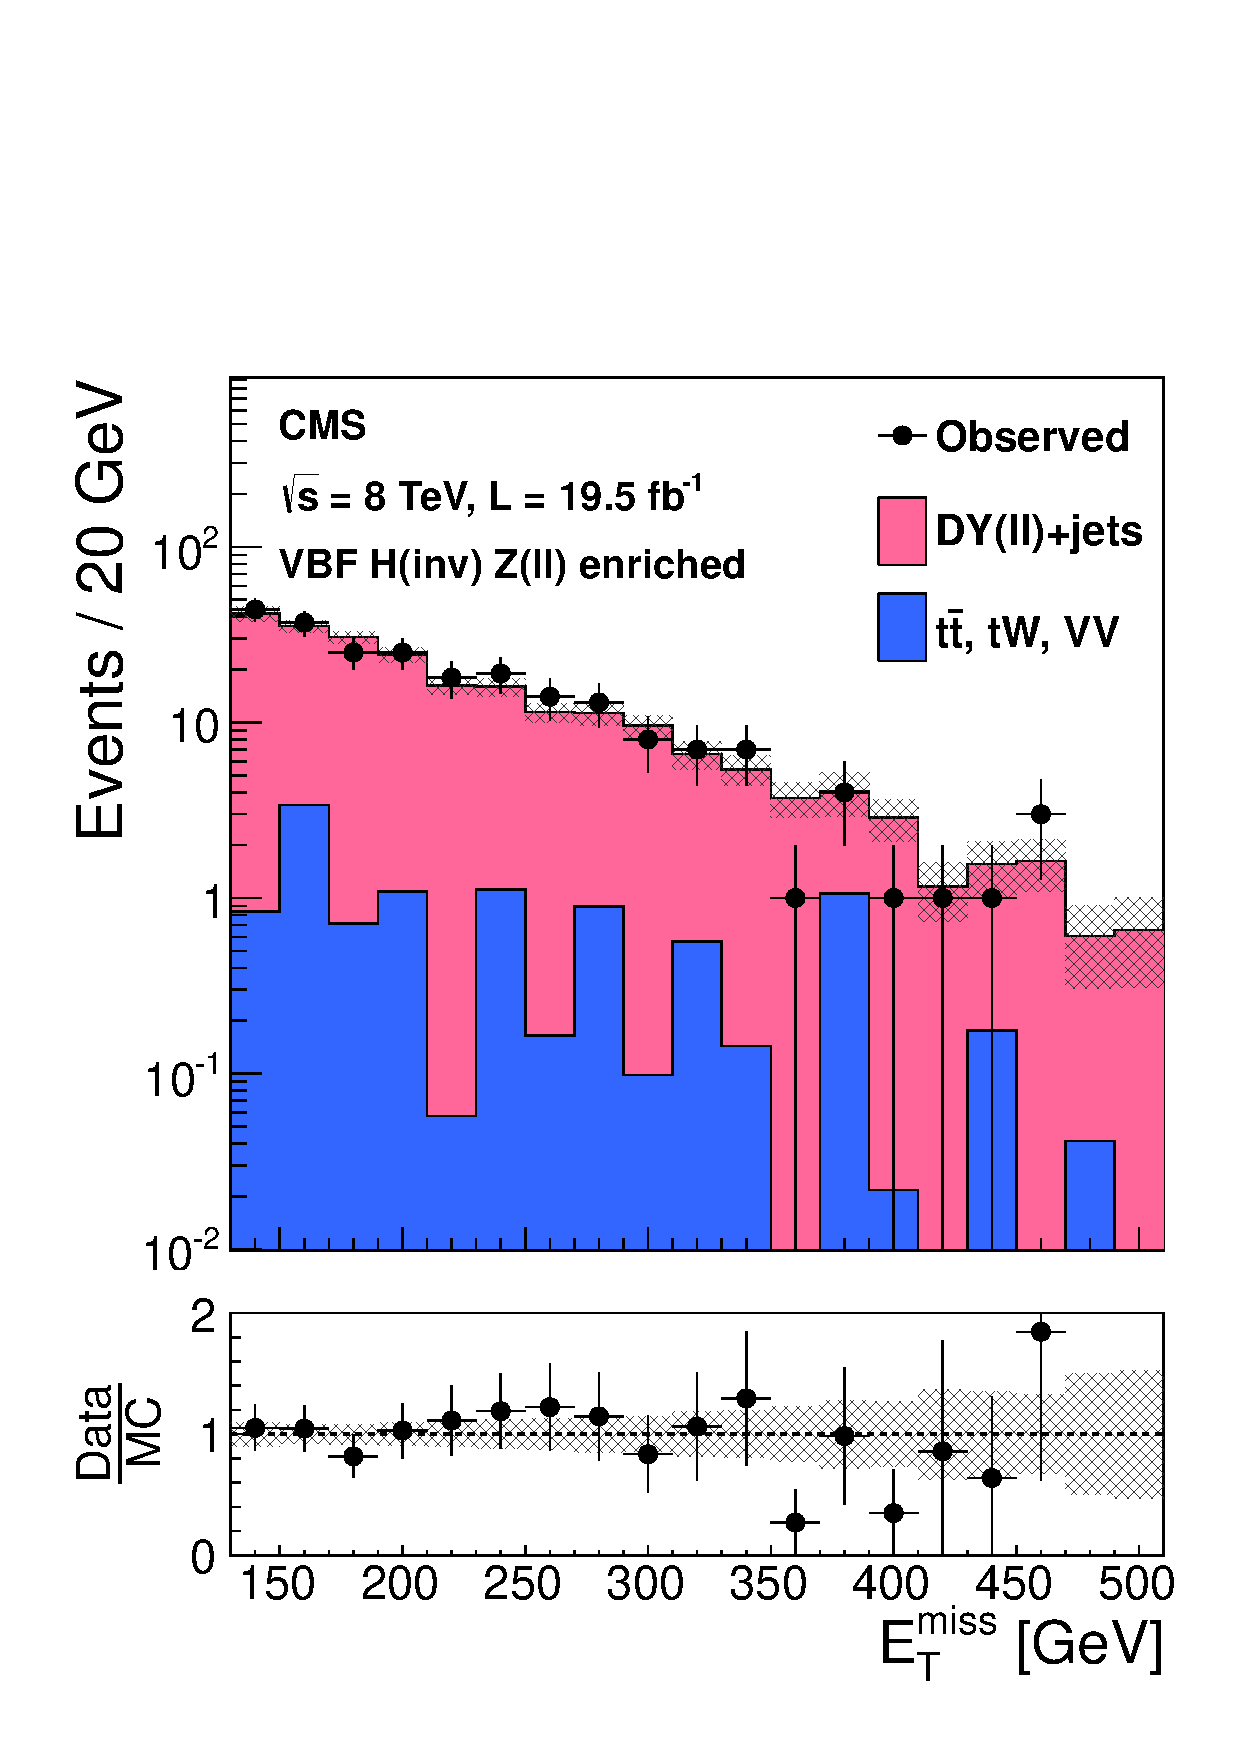
\includegraphics[width=.6\largefigwidth]{plots/prompt/VBF-ZCtrl-MET.pdf}
  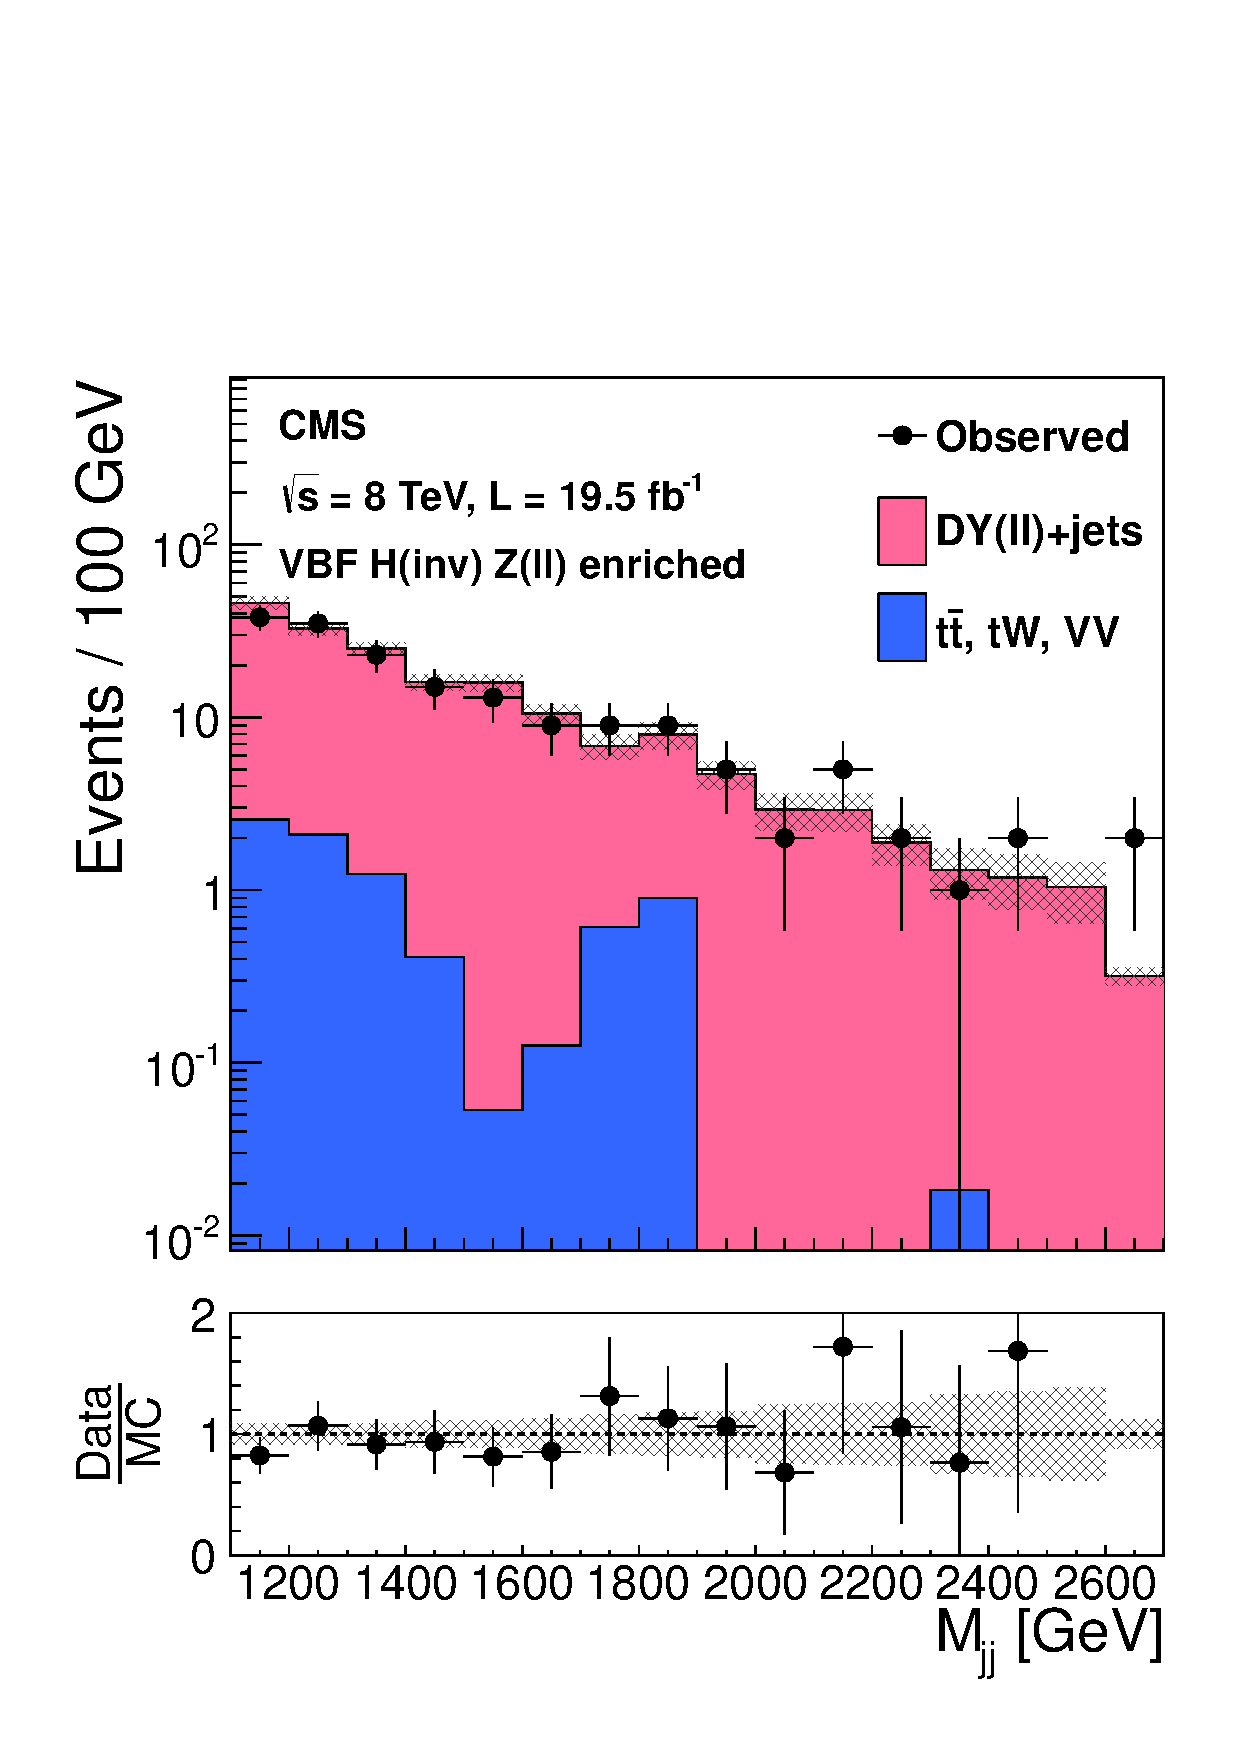
\includegraphics[width=.6\largefigwidth]{plots/prompt/VBF-ZCtrl-Mjj.pdf}
  \caption{Distributions of the \MET (left) and $M_{jj}$ (right) in a relaxed \PZ control region, with no requirement on $\Delta\phi_{jj}$, the \ac{CJV} removed, and the requirements on $M_{jj}$ and $Delta\eta_{jj}$ relaxed to 1000 \GeV and 3.5 respectively. The hatched region illustrates the systematic uncertainty~\cite{Chatrchyan:2014tja}.}
  \label{fig:promptznunu}
\end{figure}




\subsection{QCD}%??
\label{sec:promptacQCD}
%??maybe others that were tried
The \ac{QCD} multijet background remaining after the full event selection is mostly from events where jets are mismeasured. The size of the \ac{MC} samples available for studying this process is not sufficient for them to be relied upon to generate extrapolation ratios between a control region and the signal region. The remaining \ac{QCD} multijet background is therefore estimated using a so-called ``ABCD'' method. In this method four regions, A, B, C and D, are defined according to whether events pass or fail the \MET and \ac{CJV} cuts as shown in \FigureRef{fig:abcdmethod}. Region D is the signal region and regions A, B and C are three mutually exclusive control regions.

\begin{figure}
  \begin{tabular}{l|c|c|l}
    \multicolumn{1}{c}{}&\multicolumn{1}{c}{Fail \MET} & \multicolumn{1}{c}{Pass \MET} &\\
    \cline{2-3}
    Fail \ac{CJV} &\cellcolor{orange} A & \cellcolor{orange}B &\\
    \cline{2-3}
    Pass \ac{CJV} &\cellcolor{orange} C & \cellcolor{green}D &\\
    \cline{2-3}
  \end{tabular}

  \caption{A diagram of the regions used in the \ac{QCD} multijet ABCD background estimation method. Region D is the signal region and regions A, B and C are mutually exclusive control regions.}
  \label{fig:abcdmethod}
\end{figure}

The efficiency to pass the \MET and \ac{CJV} cuts can be determined from the ratios between regions A and B, and A and C respectively. The number of events expected in the signal region is then:
\begin{align}
  \label{eq:abcd}
  \begin{split}
  N_{D}&=N_{A}\cdot\frac{N_{B}}{N_{A}}\cdot\frac{N_{C}}{N_{A}}\\
  &=\frac{N_{B}\cdot N_{C}}{N_{A}}
  \end{split}
\end{align}
Where $N_{A,B,C}$ is the number of events observed in region $A,B,C$ in data minus the number expected from V+jets or other minor backgrounds, i.e. the number of events in the region believed to be from QCD. This method relies on the probability of an event passing the \ac{CJV} being uncorrelated with the \MET of the event. This has been checked by comparing the \MET distribution, below 130 \GeV\,, for events which pass and fail the \ac{CJV}. The maximum fractional difference observed between bins of these two distributions is 40\%, so this is added as a systematic to the \ac{QCD} multijet background yield.

%??Table of results

\subsection{Minor backgrounds}%??
\label{sec:promptminor}
%??from MC, doesn't matter because they're small

\section{Systematic uncertainties}%??
\label{sec:promptsyst}
%??Systematics
%??JES/JER/UES
%??Znunu extrap fac
%??lepton weights

\section{Results}%??
\label{sec:promptresults}
